\documentclass[
  oneside,
  degree=bachelor,
  field=science,
  fullwidthstop=circle,
  fontset=fandol,
  times=false,
  minted=true,
  biblatex=true,
]{tongjithesis}

\tjbibresource{bib/note.bib}

\begin{document}

% ============================================================
%  文档类选项（在 main.tex 的 \documentclass[...]{tongjithesis} 中设置）
%  field=science    理工科（工科类、理科类，默认）— 章节编号：1 / 1.1 / 1.1.1
%  field=humanities 文科  （人文、法学、外语、艺术）        — 章节编号：一、/（一）/ 1.
%  degree=bachelor  学士学位（默认）
%  degree=master   硕士学位
%  degree=doctor   博士学位
% ============================================================

% ============================================================
%  封面信息
% ============================================================
\school{国豪书院}
\major{计算机科学与技术}
\student{2251251}{姚雨萱}
\thesistitle{基于多模态大语言模型的胶质母细胞瘤候选药物分子生成与优化研究}{}
\thesistitleeng{Glioblastoma Drug Candidate Molecule Generation and Optimization Based on Multi-modal Large Language Model}{}
\thesisadvisor{关佶红\quad 教授}
\thesisdate{2026}{5}{10} % 使用当前日期; 也可以自定义日期

% ============================================================
%  信息说明页
% ============================================================

% 成果类型（三选一）：
%   thesis      — 毕业论文，摘要
%   design      — 毕业设计（软件/创意/建筑等非工程设计类），摘要
%   engineering — 毕业设计（工程设计类），设计总说明
\infotype{thesis}

% 内容简述（请用300字以内简要概述）
\infoabstract{%
本文针对胶质母细胞瘤（Glioblastoma, GBM）新药早期发现中候选分子生成难、多目标约束平衡复杂等问题，提出了一种名为 GBM-PharmaMind 的候选药物分子生成与优化框架。该框架以多模态大语言模型为基础，通过低秩适配（Low-Rank Adaptation, LoRA）微调进行胶质母细胞瘤领域知识适配，结合图扩散变换器实现分子图生成与编码，并引入思维链（Chain-of-Thought, CoT）与思维树（Tree-of-Thoughts, ToT）协同推理，引导模型在靶点信息、血脑屏障穿透性和成药性约束下生成候选分子。生成结果结合分子对接、成药性预测和结构风险检测进行评估与反馈，实现迭代优化。在代表性靶点上的实验结果表明，该框架能够生成具有一定靶点匹配潜力、血脑屏障穿透性和成药性特征的候选分子；对比实验表明，该框架在高分候选分子质量方面具有优势；消融实验说明领域知识适配、协同推理和评估反馈等模块均有助于提升生成质量。本文研究可为胶质母细胞瘤创新药物的早期虚拟筛选提供计算辅助思路。
}

% 毕业设计：图纸数量与正文字数（成果类型为 design 或 engineering 时填写，两者须同时填写）
% \infodrawings{5}
% \infowordcount{15000}

% 毕业论文：正文总字数（成果类型为 thesis 时填写）
\infothesiswords{27120}

% 随附资料（每条用 \item 开头；不填则显示空白行）
\infomaterials{
  \item GBM-PharmaMind框架源代码及简要使用说明
}

\MakeCover
\cleardoublepage
\MakeInfoPage
\cleardoublepage

\frontmatter
\MakeAbstract{
胶质母细胞瘤（Glioblastoma, GBM）是一类常见的恶性脑肿瘤。由于肿瘤异质性强，且药物较难穿过血脑屏障，GBM 新药发现仍面临较大困难。近年来，多模态大语言模型被用于分子生成和虚拟筛选，为候选药物发现提供了新的思路。传统虚拟筛选通常依赖已有化合物库。该方法流程清楚，但可探索的化学空间有限，许多疾病相关信息也难以提前进入筛选过程。大模型辅助的分子生成方法可以生成新的候选结构，但在 GBM 场景中仍存在一些问题。模型可能忽略中枢神经系统药物的设计要求，生成分子也常需要在后续评价中被大量筛除。

针对上述问题，本文设计了 GBM-PharmaMind 候选药物分子生成与优化框架。本文先创新性构建了面向GBM候选分子生成的领域知识输入方式。 随后，本文以多模态大语言模型和分子图—文本生成模型为基础，引入低秩适配（ LoRA ）进行领域适配，使模型更贴近 GBM 药物设计任务。分子生成时，本文创新性地设计了 CoT-ToT 三阶段推理策略。该策略将生成过程分为骨架提议、片段组装和 SMILES 输出三个阶段，生成后的分子会经过对接预测、成药性评估、血脑屏障预测等检查，评价结果用于反馈下一轮生成。最终候选分子的排序则依据 DrugCLIP 和 SwissADME 测得的结果完成。

本文在多个 GBM 相关靶点上进行了实验。实验结果表明，该框架能够生成具有进一步筛选价值的候选分子。对比实验和消融实验说明，领域适配、分阶段推理和评估反馈设计对生成质量都有积极作用。
}{胶质母细胞瘤；多模态大语言模型；分子生成；多目标优化}

\MakeAbstractEng{
Glioblastoma (GBM) is a common malignant brain tumor. Drug discovery for GBM remains difficult because the tumor is highly heterogeneous, and many compounds cannot easily pass through the blood-brain barrier. In recent years, multimodal large language models have been introduced into molecular generation and virtual screening, offering a new route for finding candidate drugs. Traditional virtual screening usually starts from existing compound libraries. This workflow is straightforward, but the chemical space that can be explored is limited. Disease-related information is also hard to include before screening begins. Large-model-assisted molecular generation can provide new candidate structures, but it still faces problems in the GBM setting. The model may overlook the design requirements of central nervous system drugs, and many generated molecules may be removed during later evaluation.

To address these problems, this thesis designs GBM-PharmaMind, a framework for generating and optimizing candidate drug molecules for GBM. First, GBM-related target information, clinical treatment experience, and molecular structure knowledge are collected and written into prompts. Then, based on a multimodal large language model and a molecular graph-text generation model, LoRA is used for domain adaptation so that the model can better fit the GBM drug design task. During molecular generation, this thesis adopts a CoT-ToT reasoning strategy. The generation process is divided into three stages: scaffold proposal, fragment assembly, and SMILES output. The generated molecules are then checked by docking prediction, drug-likeness evaluation, and blood-brain barrier prediction. The evaluation results are used to guide the next round of generation. The final ranking of candidate molecules is determined by the results measured with external tools, including DrugCLIP and SwissADME.

Experiments are carried out on several GBM-related targets. The results show that the proposed framework can generate candidate molecules with further screening value. Comparative experiments and ablation experiments also indicate that domain adaptation, staged reasoning, and evaluation feedback all have positive effects on generation quality.
}{Glioblastoma; Multi-modal Large Language Model; Molecular Generation; Multi-Parameter Optimization}


\clearpage
\tableofcontents
% \listoffigures   % 插图清单（根据需要取消注释）
% \listoftables    % 表格清单（根据需要取消注释）
\cleardoublepage

\mainmatter
\chapter{绪论}\label{chap:introduction}

\section{研究背景与意义}\label{sec:background}

\subsection{胶质母细胞瘤的临床挑战与药物发现难点}\label{sec:gbm-clinical}

胶质母细胞瘤（Glioblastoma, GBM）是成人中最常见且最具侵袭性的原发性恶性脑肿瘤。根据美国中央脑肿瘤登记处（Central Brain Tumor Registry of the United States, CBTRUS）的流行病学数据，GBM约占所有原发性脑肿瘤的14.9\%、所有胶质瘤的57.3\%，年发病率约为3.2/10万人口~\cite{Stupp2005}。诊断中位年龄为65岁，且男性发病率高于女性，比例约为1.6:1。

当前新诊断GBM的标准治疗方案，即Stupp方案，由Stupp等人于2005年确立，至今仍是GBM治疗的金标准~\cite{Stupp2005}。该方案包括最大程度安全手术切除，随后进行同步放疗（60 Gy，30次分割）和每日替莫唑胺（Temozolomide, TMZ）化疗（75 mg/m²/天），随后进行6-12个周期的TMZ辅助化疗。尽管采用了这种积极的多模式治疗策略，GBM患者的预后仍然极差：中位总生存期仅为12-15个月，五年生存率不足5\%，中位无进展生存期约为6-7个月，几乎所有患者都会出现肿瘤复发。

GBM极差的预后可归因于以下几个固有的生物学特征：

\textbf{分子异质性}：GBM在分子水平上表现出显著的肿瘤间和肿瘤内异质性。基于转录组分析，GBM可分为四种分子亚型：经典型（Classical）、间充质型（Mesenchymal）、前神经元型（Proneural）和神经型（Neural）~\cite{Verhaak2010}。经典型以表皮生长因子受体（Epidermal Growth Factor Receptor, EGFR）基因扩增和7号染色体扩增/10号染色体缺失为特征，而前神经元型常伴有血小板源性生长因子受体 α（Platelet-Derived Growth Factor Receptor Alpha, PDGFRA）基因改变以及异柠檬酸脱氢酶（Isocitrate Dehydrogenase, IDH）基因突变。这种分子异质性导致对靶向治疗的不同反应，使单靶点药物往往难以奏效~\cite{Verhaak2010}。

\textbf{血脑屏障挑战}：血脑屏障（Blood-Brain Barrier, BBB）是 GBM 治疗中最主要的生理障碍，限制了绝大多数化疗药物有效进入肿瘤区域~\cite{Pardridge2012}。BBB 是高度专业化的内皮结构，将循环血液与脑细胞外液分离，保护中枢神经系统免受潜在有害物质的侵害~\cite{Ferraris2020}。相关研究指出，一般给药系统较难穿透血脑屏障到达脑部病变部位，因此脑靶向递药系统和 BBB 穿透策略是脑部疾病药物研发中的重要方向~\cite{翁丹芳2021}。在严格的理化约束下，仅约 2\% 的小分子药物能够穿透 BBB 进入脑实质~\cite{Pardridge2012}：分子量（Molecular Weight, MW）需低于 400--500 Da，拓扑极性表面积（Topological Polar Surface Area, TPSA）需低于 90 Ų~\cite{Ertl2000}，脂水分配系数（LogP）需维持在 1--4 之间~\cite{Ferraris2020}，同时对氢键供体和受体数目也有严格限制。这些理化约束与靶点结合活性、代谢稳定性之间的平衡，使 GBM 药物设计成为典型的多目标优化问题。

\textbf{治疗耐药性}：GBM表现出对多种治疗模式的固有和获得性耐药~\cite{Fu2025}。TMZ耐药发生在约90\%的患者中，主要通过O6-甲基鸟嘌呤-DNA甲基转移酶（O6-Methylguanine-DNA Methyltransferase, MGMT）修复机制介导。血脑屏障限制了药物到达肿瘤部位，而肿瘤微环境促进免疫抑制和治疗耐药。

\subsection{AI驱动药物发现的机遇}\label{sec:ai-opportunity}

传统药物发现周期长、成本高（一款新药平均研发周期10-15年、成本超20亿美元）、失败率高。人工智能与药物发现的融合为加速新型治疗药物的发现提供了新的技术思路。已有研究指出，深度学习已广泛应用于药物靶标预测、药物-靶标相互作用预测、从头药物分子设计和ADMET性质预测等环节，为AI辅助新药研发提供了重要方法基础~\cite{戴青青2022}。近年来，几项与GBM药物发现挑战特别相关的人工智能技术取得了较快发展：

\textbf{大语言模型（Large Language Models, LLMs）}：基于Transformer的大语言模型的快速发展（如GPT-4、Claude，以及开源模型如LLaMA和Qwen2）展示了在自然语言理解、推理和生成方面前所未有的能力~\cite{Qwen2Team2024}。这些模型可以通过微调和领域特定知识整合来适应药物发现等科学领域~\cite{jin2025effective}。

\textbf{多模态学习}：整合文本、图像、图和其他数据模态的多模态大语言模型为复杂生物医学数据的统一表示提供了潜力~\cite{Liu2024GITMol}。在分子设计中，多模态模型可以联合处理分子结构（SMILES/SELFIES表示）、药理学描述和理化性质数据。

\textbf{图神经网络（Graph Neural Networks, GNNs）}：GNN已成为学习分子图表示的强大工具，能够准确预测分子性质和生成新型分子结构~\cite{Xu2019,Gilmer2017}。结合GNN的扩散模型在分子生成任务中显示出特别的前景~\cite{Xu2023}。

\textbf{多目标优化}：同时平衡多个药物性质的多参数优化（Multi-Parameter Optimization, MPO）方法变得越来越复杂~\cite{Zhou2019Exp}。这些方法可以导航目标亲和力、BBB通透性、代谢稳定性和毒性之间的复杂权衡空间。

\subsection{研究意义}\label{sec:research-scope}

GBM 发生在中枢神经系统，血脑屏障会限制许多药物进入脑部组织，候选药物在设计时就需要考虑脑部递送问题，分子的基础理化性质和潜在安全风险也会影响后续筛选。因此，GBM 药物设计是一个多目标约束问题，不能只围绕单一活性分数展开。

传统虚拟筛选方法通常需要预先构建化合物库，再基于该化合物库进行评价。针对胶质母细胞瘤疾病，这种做法存在几点明显不足。第一，化合物库的规模有限。许多可能对胶质母细胞瘤有效，尤其是具备血脑屏障穿透潜力的分子结构，并未预先包含在库中，导致筛选阶段无法触及这些分子。第二，胶质母细胞瘤具有较强的疾病特异性。EGFR 改变、VEGF/VEGFR 通路异常、IDH 突变等靶点背景会影响候选分子的设计方向。如果筛选过程只依赖通用化合物库，模型难以充分利用这些疾病信息。第三，胶质母细胞瘤药物设计需要较早考虑血脑屏障限制。传统流程通常在候选分子筛选完成后再进行理化性质、BBB 穿透性和结构风险等评价。这样容易出现对接结果较好，但不适合作为脑部候选药物的分子。

基于上述分析，本文构建 GBM-PharmaMind 框架，尝试在生成阶段引入胶质母细胞瘤疾病知识和计算评价反馈，使生成结果更贴近早期虚拟筛选需求。

在方法层面，本文探索了多模态大语言模型与 GBM 领域知识的结合方式，使模型在生成候选分子时能够参考疾病背景和药物设计要求。在应用层面，本文为 GBM 候选药物的早期虚拟筛选提供了一种计算辅助方案。生成结果可作为后续实验筛选的候选集合，从而减少早期发现中的盲目搜索。


\section{国内外研究现状}\label{sec:related-work}

过去十余年间，AI驱动的分子生成领域发展迅速，多种方法范式在从头药物设计中取得了显著进展。然而，现有方法在面向胶质母细胞瘤（GBM）这类特定疾病领域时，仍存在明显的能力不足。本节系统回顾相关研究现状，并分析现有方法与本文研究目标之间的差距。

\subsection{传统深度生成模型在分子生成中的应用}\label{sec:traditional-dl}

基于深度学习的分子生成方法经历了从无监督表示学习到条件生成、从单目标到多目标优化的演进历程。本小节综述主要方法范式及其在从头药物设计中的应用与局限性。

\textbf{变分自编码器（VAE）类模型}：VAE以无监督方式学习分子结构的连续潜在表示~\cite{GomezBombarelli2018}，能够从潜在空间采样生成新型分子。VAE学习的潜在空间具有平滑的插值特性，允许在潜在空间中插值采样以生成具有期望性质的分子。然而，VAE经常产生无效的分子结构~\cite{GomezBombarelli2018}，对特定分子特征的控制有限，且难以直接融入领域知识约束。在面向GBM等特定疾病领域时，VAE缺乏对疾病背景知识的理解能力。

\textbf{GAN与RNN类模型}：基于生成对抗网络（GAN）和循环神经网络（RNN）的方法~\cite{Segler2017}将分子生成建模为序列生成任务，直接在SMILES字符串空间进行操作。这类方法的优势在于可以借助强大的序列生成模型，但其生成的SMILES字符串可能存在无效性问题，且难以保证生成分子满足多维理化约束~\cite{Segler2017}。更重要的是，这类模型通常采用"先生成、后筛选"的二阶段范式，生成过程缺乏对物理约束的动态感知。

\textbf{Transformer-SMILES模型}：MolGPT使用Transformer-解码器架构进行分子生成~\cite{Bagal2021}，在基准数据集上展示了具有竞争力的性能。这类方法可以利用大规模预训练语言模型的能力，但同样面临SMILES有效性和多目标约束控制的挑战~\cite{Bagal2021}。MolGPT更偏向于无条件分子生成，而非针对特定靶点或疾病领域的条件生成。

\textbf{强化学习优化模型}：REINVENT 2.0结合了基于RNN的生成与使用行为克隆和基于记忆的策略更新的RL优化~\cite{Blaschke2020}。RL方法的优势在于可以直接优化复合目标，但奖励函数设计困难，且探索空间巨大可能导致训练不稳定~\cite{Zhou2019Exp}。在GBM等多目标约束场景下，设计能够同时平衡BBB穿透性、靶点选择性、毒性和合成可行性的奖励函数面临挑战。

\textbf{图神经网络与扩散模型}：图神经网络和图扩散模型在分子生成任务中取得了显著进展~\cite{Liu2024GraphDiffusion,Xu2023}。几何潜在扩散模型能够生成具有真实3D构象的分子~\cite{Xu2023}，Graph Diffusion Transformers在多条件分子生成方面展示了优异的性能~\cite{Liu2024GraphDiffusion}。然而，这些方法通常缺乏对自然语言描述和疾病领域知识的理解能力，难以直接用于"根据靶点描述生成候选分子"的任务。

传统深度生成模型的主要不足集中在三个方面：分子有效性不稳定、疾病知识利用不足，以及多目标约束控制能力有限。对于GBM任务而言，后一问题尤为突出，因为候选分子不仅需要满足靶点匹配，还要同时考虑BBB穿透倾向和基础安全性。

\subsection{大语言模型、多模态模型与平台型工具在分子生成中的应用}\label{sec:mllm-drug-discovery}

随着 Transformer 架构在自然语言处理领域的成功，大语言模型（Large Language Models, LLMs）逐渐向化学、生物医学和药物发现等科学领域扩展~\cite{jin2025effective}。与传统深度生成模型相比，LLM 能够处理靶点生物学描述、药物设计约束条件、疾病临床背景和实验文献等多模态自然语言信息~\cite{jin2025effective}，为知识密集型的药物发现任务提供了新的技术路径。

早期研究将分子表示为 SMILES 字符串，将化学语言建模视为自然语言处理任务~\cite{Bagal2021}。基于预训练语言模型的分子性质预测~\cite{jin2025effective}、分子描述生成~\cite{jin2025effective}和分子编辑~\cite{Li2025DrugPilot}等任务相继涌现，验证了大规模语言模型在化学领域的适用性。然而，这类方法依赖于 SMILES 序列的有效性~\cite{Bagal2021}，且难以精确控制生成分子的理化约束~\cite{jin2025effective}，在结构多样性和物理合理性方面存在明显不足。

针对上述问题，化学指令微调（Chemical Instruction Tuning）和领域适配技术被引入~\cite{Yu2024}。例如，Yu 等人~\cite{Yu2024}基于 Mistral-7B 构建了大规模化学指令微调数据集 LlaSMol，显著提升了模型在化学问答和性质预测任务上的表现；Jin 等人~\cite{jin2025effective}将思维链（Chain-of-Thought, CoT）推理引入分子性质预测，增强了模型的可解释性。然而，这些方法在面向特定疾病靶点生成候选分子时，仍缺乏对疾病生物学背景、靶点作用机制和药物递送约束的充分建模~\cite{jin2025effective}。

多模态分子生成模型将分子图、SMILES、蛋白口袋结构和药物文本描述映射到统一的语义表示空间~\cite{Liu2024GITMol,Li2025ChemVLM}，为跨模态条件生成提供了基础~\cite{Liu2024GITMol,Li2025ChemVLM}。GIT-Mol~\cite{Liu2024GITMol}在统一框架内处理图形、图像和文本分子科学数据；ChemVLM~\cite{Li2025ChemVLM}探索了视觉-语言模型在化学领域的零样本和少样本学习能力；DrugPilot~\cite{Li2025DrugPilot}将 LLM 与多种工具数据库集成，支持复杂的多步推理链。其中，Liu 等人~\cite{liu2025multimodal}提出的 Llamole 将大语言模型的语义理解能力与图扩散变换器的分子图生成能力相结合~\cite{liu2025multimodal}，在受控分子生成和逆合成规划任务上取得了优于 14 个基线模型的表现~\cite{liu2025multimodal}。这种图—文本协同生成架构更契合"根据靶点描述生成候选分子"的药物设计任务~\cite{liu2025multimodal}。

平台型分子设计工具通常集成分子生成、性质预测和结构优化等功能~\cite{rusinko2024aiddison,torrensfontanals2024playmolecule}，具有使用门槛低、交互便捷和部署成熟等优点~\cite{rusinko2024aiddison,torrensfontanals2024playmolecule}，适合快速探索候选分子。然而，这类工具普遍存在模型细节不透明、可解释性和可控性有限等问题~\cite{wong2025explainable}，难以灵活引入特定疾病的多模态知识库~\cite{Li2025DrugPilot}；此外，平台型工具在生成分子时容易出现骨架收敛现象~\cite{Brown2019,varela2020skeledock}，即围绕少数已知母核进行局部修饰，化学空间探索范围有限~\cite{Brown2019}，更难与外部物理评估工具集成形成闭环反馈~\cite{Li2025DrugPilot}。

尽管大语言模型与多模态方法在分子生成任务中取得了显著进展~\cite{jin2025effective,Li2025DrugPilot}，但在以下方面仍存在不足：（1）事实可靠性不足，LLM 可能生成化学无效结构或错误信息；（2）化学有效性难以稳定保证~\cite{jin2025effective}；（3）物理约束难以精确控制~\cite{jin2025effective}；（4）在 GBM 等特定疾病场景下，还需同时满足靶点匹配能力、BBB 穿透倾向和基础成药性的多目标约束~\cite{Pardridge2012}。上述挑战构成了本文方法研究的核心动机。

\subsection{GBM靶向药物发现与CNS成药性挑战}\label{sec:gbm-drug-development}

GBM 药物发现面临的核心挑战，使其与其他肿瘤药物设计存在明显区别。主要体现在以下几个方面。

\textbf{EGFR 是 GBM 中研究较多的靶点。} EGFR及其突变体 EGFRvIII 在 GBM 中较为常见，已有较多 EGFR 抑制剂结构和母核信息被公开。多种 EGFR 酪氨酸激酶抑制剂也曾用于 GBM 相关临床研究。然而，由于血脑屏障限制和旁路信号激活等因素，EGFR 靶向疗法的效果仍然有限。这提示 EGFR 候选分子设计不能只关注靶点抑制作用，还需要考虑中枢神经系统成药性。

\textbf{VEGF/VEGFR 通路与 GBM 相关血管生成过程密切相关。} GBM 的生长和侵袭与血管生成密切相关，因此 VEGF/VEGFR 通路也是重要研究方向。抗 VEGF 治疗在复发性 GBM 中已有应用，但在总体生存获益方面仍存在局限。这说明，仅抑制血管生成往往不足以控制 GBM 进展。对于 VEGF/VEGFR 靶点，候选分子设计还需要面对结合机制复杂、疗效持续性不足等问题。

\textbf{IDH1/IDH2 突变是 GBM 的重要分子标志。} IDH 突变会导致异常代谢产物积累，并影响 GBM 的分子分型。相较于部分通路靶点，IDH1 突变体的结构口袋较为明确，因此更适合用于对接评价和候选分子筛选。但 IDH1/IDH2 突变并不适用于所有 GBM 患者，所以较高的计算评分不能直接说明其具有广泛临床适用性。

\textbf{血脑屏障是 GBM 药物设计中的主要限制。} GBM 位于中枢神经系统，候选药物需要进入脑部病灶区域才可能发挥作用。血脑屏障会阻止许多外源分子进入脑组织，使不少体外活性较好的分子难以到达有效部位。因此，GBM 候选分子在设计时需要考虑分子量、极性表面积、脂溶性等理化性质。实际穿透能力还会受到主动转运、外排泵和代谢稳定性等因素影响，简单描述符难以完全反映真实情况。

\textbf{GBM 的异质性会削弱单一靶点策略的效果。} GBM 在分子水平上存在明显差异，不同亚型和突变背景会影响治疗反应。单一靶点药物往往难以覆盖全部患者，也容易受到耐药机制影响。因此，GBM 候选分子设计不能只优化某一个指标，还需要综合考虑靶点作用、BBB 相关性质和基础安全性。

综上，GBM 药物发现不仅是普通肿瘤靶向药物设计的延伸。其特殊性来自疾病本身的分子背景，也来自中枢神经系统药物递送限制。如果生成模型缺少这些信息，后续筛选中容易出现大量价值有限的候选分子。这也是本文引入 GBM 领域知识、分阶段生成策略和计算评价反馈的原因。


\section{研究内容}\label{sec:research-content}

本文围绕"如何利用多模态大语言模型生成具有GBM治疗潜力的候选药物分子"展开。研究内容主要包括三个方面：

首先，构建面向GBM候选分子生成的多模态知识输入机制，将靶点信息、临床治疗经验、参考分子和结构约束转化为模型可调用的信息。这一部分需要回答的问题是：如何有效融合GBM病理背景、药理特性、分子结构与生物活性信息，建立统一的多模态表征空间。

其次，基于Qwen2-7B-Instruct与Llamole~\cite{liu2025multimodal}构建GBM-PharmaMind框架，并结合LoRA适配~\cite{hu2022lora}和CoT-ToT推理~\cite{Wei2022,Yao2023}实现候选分子生成。这一部分需要回答的问题是：如何引导多模态大语言模型根据复杂的多目标约束（BBB穿透性、靶点选择性、药代动力学性质）进行可控的分子生成。

最后，利用AutoDock Vina~\cite{Trott2010}、BBB经验预测、DILI/hERG结构警报~\cite{Aronov2008}和MPO Reward建立生成结果的计算评价与反馈机制。这一部分需要回答的问题是：如何建立生成分子的快速、可靠虚拟验证体系，实现生成与评估的闭环反馈。


\section{本文所做工作}\label{sec:research-work}

本文围绕胶质母细胞瘤候选药物分子的早期计算生成问题展开研究。GBM 药物发现与普通分子生成任务不同，模型既要理解疾病相关靶点信息，也要考虑中枢神经系统药物设计中的血脑屏障限制。传统虚拟筛选方法通常依赖已有化合物库，筛选空间容易受到限制。通用分子生成模型虽然可以产生新的候选结构，但如果缺少 GBM 疾病背景和后续评价反馈，生成结果可能不符合实际筛选要求。基于这一问题，本文构建了 GBM-PharmaMind 候选药物分子生成与优化框架。

本文所做工作和创新点主要包括以下四个方面。

（1）构建了面向 GBM 候选分子生成的领域知识输入机制。该部分的创新性在于，将GBM靶点背景、CNS药物设计规则和结构风险提示提前写入生成输入，而不是在候选分子生成后再统一筛除。本文整理了 GBM 相关靶点信息、临床治疗经验、参考分子结构和中枢神经系统药物设计规则，并将这些内容转化为模型可使用的提示信息。通过这种方式，模型在生成候选分子时可以参考 EGFR、VEGF/VEGFR 和 IDH1/IDH2 等靶点背景，也可以提前考虑血脑屏障相关的理化要求。

（2）首次提出GBM-PharmaMind候选药物分子生成与优化框架。该框架将多模态大语言模型、分子图—文本生成模型、LoRA领域适配和物理评估反馈连接到同一流程中，使GBM候选分子生成不再局限于通用SMILES生成。以多模态大语言模型和分子图—文本生成模型为基础，引入 LoRA 进行 GBM 领域适配，使模型更贴近胶质母细胞瘤药物设计任务。相比直接使用通用模型生成 SMILES，该方法能够将疾病信息、文本描述和分子结构生成过程联系起来，从而提高候选分子生成的针对性。

（3）设计了面向GBM候选分子生成的CoT-ToT三阶段推理策略。本文将候选分子生成拆分为骨架提议、片段组装和SMILES输出三个阶段，并在每一阶段保留多个候选方向，以减少单一路径生成带来的局部收敛问题。CoT（Chain-of-Thought）用于引导模型按照较清晰的设计步骤进行推理，ToT（Tree-of-Thoughts）用于保留多个候选方向，避免生成过程过早局限在单一路径中。该策略使候选分子的生成过程更容易被检查和调整。

（4）建立了面向GBM候选分子生成过程的计算评价与反馈机制。该机制将Vina对接、BBB预测、成药性评估和结构风险检查用于生成阶段的反馈与剪枝，并在最终阶段依据DrugCLIP和SwissADME相关结果完成候选分子排序。生成阶段的评价结果会反馈到后续生成过程中，用于减少明显不符合要求的候选结构。最终候选分子的排序则依据 DrugCLIP 和 SwissADME 测得的结果完成。实验结果表明，领域适配、分阶段推理和评估反馈设计对生成质量都有积极作用。


\section{论文结构}\label{sec:structure}

本文共分为五章。第1章介绍GBM候选药物发现的研究背景、现有方法不足和本文主要工作。第2章梳理大语言模型、分子表示、图生成模型、LoRA、CoT-ToT推理和物理评估等相关技术。第3章给出GBM-PharmaMind框架设计，包括知识库、Prompt生成器、LoRA适配、CoT-ToT生成算法和物理反馈机制。第4章展示实验设置、主实验结果、对比实验和消融实验。第5章总结本文工作，分析方法不足，并讨论后续改进方向。

\chapter{相关技术与理论基础}\label{chap:theory}

\section{引言}\label{sec:ch2-intro}

本章主要介绍本文研究所涉及的相关技术与理论基础。候选药物分子生成任务涉及深度学习、自然语言处理、分子表示学习和生成模型等多个方向，因此有必要对后续研究中使用的关键技术进行梳理。本章将围绕大语言模型、分子表示与多模态对齐、分子生成模型、CoT-ToT推理、物理评估方法以及LoRA参数高效微调等内容展开介绍，为第3章的框架设计和第4章的实验分析奠定理论基础。

\section{面向药物分子生成的大语言模型}\label{sec:llm-for-molecular-design}

大语言模型不仅可用于文本生成，还可在任务理解、条件建模和生成过程控制等方面发挥作用。在分子生成任务中，LLM能够对靶点描述、理化约束和药物设计要求进行语义理解，并为后续分子结构生成提供条件信息。

\subsection{大语言模型在分子生成任务中的作用}

传统分子生成模型（如VAE、GAN、扩散模型）通常以“分子图”或“SMILES序列”作为直接输入~\cite{GomezBombarelli2018,Bagal2021}，缺乏对自然语言描述的语义理解能力。然而，药物设计任务的本质是根据靶点信息、疾病背景、理化约束、风险提示等文本描述，生成满足多维约束的分子结构。

上述药物设计任务的文本驱动特性，决定了分子生成系统需要具备语义理解、多模态对齐、结构化推理和工具调用等多方面能力。具体而言，系统应能理解"EGFR靶点""BBB穿透性""TPSA<90"等药物设计专业描述，并将文本语义与分子结构（SMILES、分子图）进行对齐~\cite{Wei2022}；同时，系统还需具备按逻辑顺序拆解分子设计任务的能力~\cite{Wei2022}，并能够调用物理评估工具获取反馈~\cite{Li2025DrugPilot}。大语言模型具备上述能力~\cite{Qwen2Team2024,jin2025effective}，因此成为分子生成系统的核心组件~\cite{jin2025effective,Li2025DrugPilot}。

\subsection{LLM在分子生成中的角色定位}

在 GBM-PharmaMind 框架中，基于 Qwen2-7B-Instruct~\cite{Qwen2Team2024} 的大语言模型承担多重角色：作为任务规划器，将"生成GBM靶向候选分子"这一模糊目标分解为靶点分析、骨架选择、药效团设计、ADMET评估和SMILES输出等结构化步骤~\cite{Wei2022}；作为 Prompt 解释器，理解 GBM 知识库中的靶点信息、理化约束和风险提示，并将其转化为分子生成的条件；作为多模态生成控制器，协调分子图生成（通过图扩散变换器）和 SMILES 输出~\cite{liu2025multimodal}，实现文本语义到分子结构的映射；作为反馈整合器，将物理评估结果（Vina 对接、BBB 评分、毒性警报）整合到下一轮 Prompt 中~\cite{Yao2023}，引导生成方向的动态调整。

\subsection{LLM单独用于分子生成的局限性}

然而，LLM 单独用于分子生成时存在明显局限：生成的 SMILES 可能存在化学无效结构~\cite{Bagal2021}，难以精确遵循 MW、LogP、TPSA 等理化数值约束~\cite{Pardridge2012}，且无法自主评估生成分子的理化性质和对接分数~\cite{Trott2010}。因此，LLM 必须与分子图模型（RNN、GNN、扩散模型）和外部评估工具（Vina、ADMET 预测）结合~\cite{Li2025DrugPilot}，形成完整的生成-验证闭环。

\section{分子表示与多模态对齐}\label{sec:molecular-representation}

分子可以用不同的表示方式进行编码，每种表示方式捕获了不同层面的化学信息~\cite{Gilmer2017}。理解这些表示方法的优缺点，是设计分子生成系统的基础。

\subsection{SMILES表示的优缺点}

SMILES（Simplified Molecular Input Line Entry System）是一种基于字符串的分子表示方法，能够将分子图编码为一条 ASCII 字符串，并通过原子符号、键符号和分支括号表示分子的拓扑结构~\cite{Weininger1988}。这种表示方法具有紧凑性，例如苯分子的 SMILES 表示为 "c1ccccc1"，便于存储和传输；同时，其序列形式与自然语言处理技术天然兼容，可直接使用 Transformer 或 RNN 处理~\cite{Bagal2021}。然而，SMILES 也存在固有缺陷：同一分子可能对应多种不同的字符串表示，字符串中的微小扰动可能导致生成结果无效~\cite{Bagal2021}，且缺乏直观的几何意义，难以直接反映分子的三维构象。

SELFIES（SELF-referencing Embedded Strings）通过引入"引用"机制，使任意SELFIES字符串必然对应一个有效的分子~\cite{KrenNips2020}，从而提升了生成模型的有效率~\cite{KrenNips2020}。

\subsection{分子图表示的优势}

分子图（Molecular Graph）将分子表示为数学图$G = (V, E)$，其中节点集合$V$代表原子，边集合$E$代表化学键，能够较好地保留分子的拓扑结构信息~\cite{Xu2019}。与 SMILES 序列相比，分子图在结构表达上更加直观，原子和化学键之间的关系能够被完整保留；同时，节点特征和边特征可分别编码原子类型、价电子数、电负性、键类型和芳香性等化学信息~\cite{Gilmer2017}。此外，分子图与图神经网络天然兼容，后者可以通过消息传递机制聚合局部结构信息，从而有效学习分子表示~\cite{Xu2019,Gilmer2017}。

在多模态分子生成中，SMILES和分子图各有优势~\cite{liu2025multimodal}：SMILES便于语言模型处理，分子图便于图神经网络处理~\cite{liu2025multimodal}。Llamole~\cite{liu2025multimodal}的核心设计正是将两者结合，实现文本—分子对齐~\cite{liu2025multimodal}。本文在Llamole的基础上构建GBM-PharmaMind框架，进一步整合领域知识注入和物理评估反馈。

\subsection{多模态对齐在分子生成中的作用}

蛋白-分子匹配任务本质上是一个跨模态任务~\cite{Gao2023}：输入是蛋白口袋结构（3D几何信息）和靶点描述（文本语义），输出是分子结构（2D图或SMILES）。具体而言，系统需要能够将"EGFR 激酶域 ATP 结合位点"~\cite{Fu2025}等靶点描述转化为分子生成条件，将 MW、LogP、TPSA 等理化约束~\cite{Ertl2000,Pardridge2012}转化为分子图的生成条件，并将文本语义和分子图映射到统一向量空间~\cite{Gao2023}，实现语义级的生成分子匹配。

DrugCLIP~\cite{Gao2023}通过对比学习将蛋白口袋和分子映射到统一向量空间~\cite{Gao2023}，为分子生成提供了语义级的评价依据~\cite{Gao2023}。Llamole~\cite{liu2025multimodal}则通过触发Token机制和语义查询Token~\cite{liu2025multimodal}，实现文本语义到分子图生成的映射~\cite{liu2025multimodal}。GBM-PharmaMind框架在此基础上进一步整合了领域知识注入和物理评估反馈机制。

\section{分子生成模型的发展与 Llamole 的适用性分析}\label{sec:generation-models}

分子生成模型经历了从VAE/GAN到Transformer，再到扩散模型和多模态LLM的演进~\cite{Grisoni2023}。本节分析各类模型的特点，并说明本文底层生成模型选择Llamole~\cite{liu2025multimodal}作为分子图—文本协同生成基础，以及在此基础上构建GBM-PharmaMind框架的依据。

\subsection{SMILES生成模型的局限}

早期分子生成模型（如 VAE~\cite{GomezBombarelli2018}、RNN~\cite{Segler2017}、MolGPT~\cite{Bagal2021}）直接在 SMILES 字符串空间进行操作，面临三重困难：SMILES 字符串的微小扰动可能导致无效结构~\cite{Bagal2021}，难以保证生成分子满足多维理化约束~\cite{Grisoni2023}，且缺乏对分子拓扑结构的显式建模~\cite{Xu2019}。

\subsection{图生成模型的优势}

图神经网络和图扩散模型在分子生成任务中取得了显著进展~\cite{Liu2024GraphDiffusion,Xu2023}。相比 SMILES 生成模型，图生成模型的优势在于：分子图表示保留了完整的拓扑结构信息~\cite{Xu2019}，节点和边的特征可编码丰富的化学知识~\cite{Gilmer2017}，扩散模型（如 Graph Diffusion Transformers~\cite{Liu2024GraphDiffusion}）支持多条件生成~\cite{Liu2024GraphDiffusion}。然而，图生成模型通常缺乏对自然语言描述的理解能力~\cite{liu2025multimodal}，难以直接用于根据靶点描述生成候选分子的任务~\cite{liu2025multimodal}。

\subsection{扩散模型在化学空间探索中的作用}

几何潜在扩散模型能够生成具有真实 3D 构象的分子~\cite{Xu2023}，其优势在于生成质量高且多样性好~\cite{Xu2023}，不易陷入模式坍塌~\cite{Liu2024GraphDiffusion}，且支持条件生成~\cite{Liu2024GraphDiffusion}，适合探索复杂的化学空间~\cite{Xu2023}，而 LLM 适合理解和分解任务~\cite{Wei2022,Yao2023}。两者的结合（Llamole~\cite{liu2025multimodal}）可以发挥各自优势~\cite{liu2025multimodal}。本文在 Llamole 的基础上构建 GBM-PharmaMind 框架，进一步整合领域知识注入和物理评估反馈。

\subsection{Llamole 模型的适用性分析}

Llamole~\cite{liu2025multimodal}是专门为逆分子设计及逆合成规划设计的多模态大语言模型~\cite{liu2025multimodal}。具体而言，Llamole 通过触发 Token 机制~\cite{liu2025multimodal}具备文本—分子对齐能力，能够理解分子设计任务的文本描述~\cite{liu2025multimodal}；通过整合图扩散变换器~\cite{Liu2024GraphDiffusion}和 GNN 编码器~\cite{Gilmer2017}支持分子图生成~\cite{liu2025multimodal}；支持逆合成路线规划~\cite{liu2025multimodal}，是评估分子合成可行性的重要环节；并将 LLM 语义理解~\cite{Qwen2Team2024}和图模型结构生成~\cite{Liu2024GraphDiffusion}深度融合~\cite{liu2025multimodal}，形成多模态融合架构~\cite{liu2025multimodal}。

原始Llamole并非专门面向GBM或CNS药物设计~\cite{liu2025multimodal}，缺少GBM领域知识注入和BBB约束处理机制~\cite{liu2025multimodal}。本文在Llamole的基础上构建GBM-PharmaMind框架，增加GBM知识库~\cite{Fu2025,Pardridge2012}和领域LoRA微调~\cite{hu2022lora}，实现面向GBM的分子生成。

\section{CoT-ToT 在分子设计中的作用}\label{sec:cot-tot-molecular-design}

Chain-of-Thought（CoT）和Tree-of-Thoughts（ToT）是提升LLM推理能力的两种策略~\cite{Wei2022,Yao2023}。本节阐述它们在分子设计中的具体作用。

\subsection{结构化推理在分子设计中的作用}

分子设计是一个多约束、多阶段的复杂任务~\cite{Zhou2019Exp}。不考虑BBB穿透性、靶点选择性、药代动力学性质~\cite{Pardridge2012}等多维约束~\cite{Zhou2019Exp}，模型可能生成理化性质不合格或化学结构无效的分子~\cite{Bagal2021}。

CoT推理~\cite{Wei2022}可以将"生成GBM靶向候选分子"这一模糊目标~\cite{Wei2022}，分解为以下结构化步骤：

具体而言，CoT 推理可将分子生成分解为：靶点分析（理解 EGFR/VEGF/IDH1 等靶点的生物学背景和结合位点特征）、骨架设计（选择具有 BBB 穿透潜力的母核结构）、药效团设计（设计 ATP 竞争性结合基团或变构调节基团）、ADMET 考虑（评估 BBB、毒性风险和代谢稳定性）和 SMILES 输出（给出最终分子结构）。这种分步推理~\cite{Wei2022}使得每一步的输出可以独立验证~\cite{Wei2022}，而非一次性生成难以检验的完整分子~\cite{Wei2022}。

\subsection{多分支搜索在候选分子探索中的作用}

CoT是线性的~\cite{Yao2023}：每个步骤只产生一个输出。单一推理路径可能限制候选结构的多样性，使模型在生成过程中陷入局部最优，从而忽略其他具有潜力的分子设计方向~\cite{Yao2023}。

ToT~\cite{Yao2023}通过多分支搜索~\cite{Yao2023}解决这一问题。具体而言，在 ToT 中骨架阶段生成 3 个候选骨架（如喹唑啉类、吲哚类、氮杂环类），片段阶段为每个骨架提供 3 个片段修饰方案，SMILES 阶段为每个片段方案生成多个候选。这种分层搜索策略~\cite{Yao2023}在探索广度和深度之间取得平衡~\cite{Yao2023}：广度保证不遗漏有潜力的设计方向，深度保证每个方向能生成具体分子。

\subsection{ToT 与剪枝的协同作用}

ToT的价值不仅在于多分支探索~\cite{Yao2023}，还在于与物理评估剪枝的协同~\cite{Yao2023}。在每个ToT阶段，低评分分支可以被提前剪除~\cite{Yao2023}，从而将更多计算资源分配给高潜力方向~\cite{Yao2023}。

例如，在骨架提议阶段，如果某个骨架的BBB预测评分较低~\cite{Clark2000}，该分支可以被提前终止~\cite{Yao2023}，避免在该方向上浪费后续的片段组装和SMILES生成计算~\cite{Yao2023}。这种"早剪枝"策略~\cite{Yao2023}显著提升了生成效率~\cite{Yao2023}。

\section{物理评估与剪枝机制}\label{sec:physics-pruning}

物理评估是分子生成系统中不可或缺的环节~\cite{Trott2010,Clark2000,Aronov2008}。本节阐述物理评估在本文框架中的定位和作用。

\subsection{物理评估在分子生成中的作用}

如前所述，LLM 单独用于分子生成时存在化学有效性~\cite{Bagal2021}和物理约束~\cite{Pardridge2012}难以保证的问题~\cite{jin2025effective,Li2025DrugPilot}。分子对接是虚拟筛选中的重要计算方法，可通过模拟小分子与药物靶标之间的相互作用，从候选化合物库中快速筛选潜在活性分子，从而提高筛选效率并降低药物发现成本~\cite{张煜卓2017}。物理评估模块通过 AutoDock Vina 对接分数~\cite{Trott2010}评估生成分子与靶点蛋白的空间匹配程度，通过 BBB 经验评分~\cite{Clark2000,Ertl2000}判断分子是否具有 CNS 药物理化倾向，通过 DILI/hERG/PAINS 警报~\cite{Aronov2008}排除具有明显风险结构的分子。这些评估主要作为生成过程中的剪枝评价指标，而非最终实验验证。

\subsection{生成阶段剪枝与最终候选排序的区分}

本文将相关评估指标分为两类不同用途：生成阶段反馈指标（Vina 对接分数和 BBB 经验评分）主要用于生成过程中的物理评估、过滤和剪枝~\cite{Trott2010,Clark2000}，帮助模型在生成过程中避免明显不适合 GBM/CNS 药物设计的结构~\cite{Trott2010,Clark2000}，属于中间反馈而非最终排序依据。最终候选分子的排序依据为离线计算得到的 TotalScore。TotalScore 综合 DrugCLIP 预测活性并计算的 Vina 对接分数、SwissADME 网站返回 BBB 穿透性预测、SA/类药性指标、PAINS/Brenk 结构警报、P-gp 风险等基础理化性质信息。DrugCLIP 和 SwissADME 是 TotalScore 的重要信息来源，但非唯一依据。二者在使用阶段和评价目的上存在差异：Vina 对接分数和 BBB 经验公式是生成-剪枝循环中的反馈信号~\cite{Trott2010,Clark2000}，而 TotalScore 中的 DrugCLIP、Vina、BBB 等各项则是最终候选分子的综合排序依据。

\subsection{物理评估的局限性}

具体而言，Vina 对接分数是经验打分~\cite{Trott2010}，\textit{不等同于实验结合自由能}，仅反映在当前打分函数和对接着眼下的相对稳定性~\cite{Trott2010}；BBB 经验公式仅考虑 TPSA 和 LogP~\cite{Clark2000}，未考虑主动转运（P-gp 等外排泵）和代谢稳定性等因素，预测结果可能与实际 BBB 穿透性存在较大偏差~\cite{Pardridge2012}。因此，所有物理评估指标仅用于早期虚拟筛选和候选分子排序参考~\cite{Trott2010,Clark2000,Gao2023}，不能替代体外活性、毒性和BBB渗透实验验证~\cite{Trott2010,Pardridge2012}。

\section{LoRA 参数高效微调}\label{sec:lora-purpose}

大语言模型的全量微调需要更新模型的所有参数，计算和存储开销巨大~\cite{hu2022lora}。LoRA~\cite{hu2022lora}通过低秩矩阵适应~\cite{hu2022lora}，在保持预训练模型能力的同时~\cite{hu2022lora}，实现领域适配~\cite{hu2022lora}。

\subsection{领域适配在分子生成任务中的作用}

通用大语言模型（如Qwen2~\cite{Qwen2Team2024}）虽然在语言理解方面表现出色~\cite{Qwen2Team2024}，但缺乏对GBM疾病背景~\cite{Fu2025}、CNS药物设计约束~\cite{Pardridge2012}和特定靶点知识~\cite{Fu2025}的深度理解。具体而言，领域适配的作用包括：通过领域适配，模型可以更好地学习 GBM 靶点相关的分子设计约束，例如 EGFR 的 EGFRvIII 变体及其相关旁路信号激活~\cite{Fu2025}。同时，模型也能更充分地利用 CNS 药物中与 BBB 相关的理化要求，如 MW<450 Da、TPSA<90 Ų 等~\cite{Ertl2000,Pardridge2012}。对于特定骨架和药效团的生成偏好，领域适配也能起到一定的引导作用。
领域LoRA微调~\cite{hu2022lora}使得模型既能利用GBM领域知识~\cite{hu2022lora}，又能保持对通用分子生成任务的能力~\cite{hu2022lora}。

\subsection{LoRA 在本文中的配置}

在本文中，LoRA~\cite{hu2022lora}的各参数含义如下：在本文配置中，$r=16$ 为秩参数，表示低秩矩阵的秩~\cite{hu2022lora}，过小会限制表示能力，过大则增加训练开销；lora\_alpha=32 为缩放因子，用于缩放 LoRA 分支的输出贡献~\cite{hu2022lora}；lora\_dropout=0.05 为丢弃率，用于防止过拟合~\cite{hu2022lora}；目标模块覆盖 Transformer 中所有线性层~\cite{hu2022lora}。

LoRA适用于本文场景的原因包括：（1）保留预训练模型的通用能力~\cite{hu2022lora}；（2）在消费级GPU（如RTX 3090）上可完成训练~\cite{hu2022lora}；（3）可以针对不同任务训练多个LoRA适配器~\cite{hu2022lora}，实现模型的灵活扩展~\cite{hu2022lora}。

\section{本章小结}\label{sec:ch2-summary}

本章围绕本文研究所需的关键技术进行了介绍。

具体而言：大语言模型承担任务规划、Prompt 解释、多模态控制和反馈整合的角色~\cite{Qwen2Team2024,jin2025effective}，但单独使用时存在化学有效性和物理约束难以保证的问题~\cite{jin2025effective,Li2025DrugPilot}；SMILES 便于语言模型处理~\cite{Weininger1988}，分子图便于图神经网络处理~\cite{Xu2019,Gilmer2017}，多模态对齐是实现文本—分子映射的关键~\cite{liu2025multimodal,Gao2023}；Llamole~\cite{liu2025multimodal}同时具备文本理解和分子图生成能力~\cite{liu2025multimodal}，是本文选择的底层生成模型~\cite{liu2025multimodal}，本文在其基础上构建 GBM-PharmaMind 框架，进一步整合领域知识注入和物理评估反馈；CoT 用于分步结构化推理~\cite{Wei2022}，ToT 用于多分支搜索~\cite{Yao2023}，两者协同实现推理方向正确与探索空间充分的平衡~\cite{Yao2023}；Vina 对接和 BBB 经验公式是生成阶段剪枝反馈~\cite{Trott2010,Clark2000}，而非最终排序依据~\cite{Trott2010,Clark2000,Daina2017}；LoRA~\cite{hu2022lora}用于实现 GBM 领域知识注入~\cite{hu2022lora}，使通用模型适配 CNS 药物设计任务~\cite{hu2022lora}。

上述技术共同构成了后续GBM候选分子生成框架的理论基础。

\chapter{基于多模态大语言模型的GBM候选分子生成框架}\label{chap:framework}

\section{引言}\label{sec:ch3-intro}

本章系统阐述GBM-PharmaMind候选分子生成框架的设计理念与具体实现。3.2节说明系统总体架构与设计思路；3.3节至3.6节分别介绍GBM多模态知识库、Prompt生成器、分子图—文本协同生成模块和GBM领域LoRA适配；3.7节给出CoT-ToT协同生成算法；3.8节与3.9节进一步说明物理评估反馈机制和最终候选分子排序机制。

\section{系统总体架构与设计思路}\label{sec:system-arch}

本文提出了GBM-PharmaMind框架，以具备分子图—文本协同生成能力的多模态大模型Llamole为基础[24]，实现了涵盖知识引导、多模态生成、物理验证和反馈调整的端到端流水线。系统架构如图3.1所示。

\begin{figure}[htbp]
    \centering
    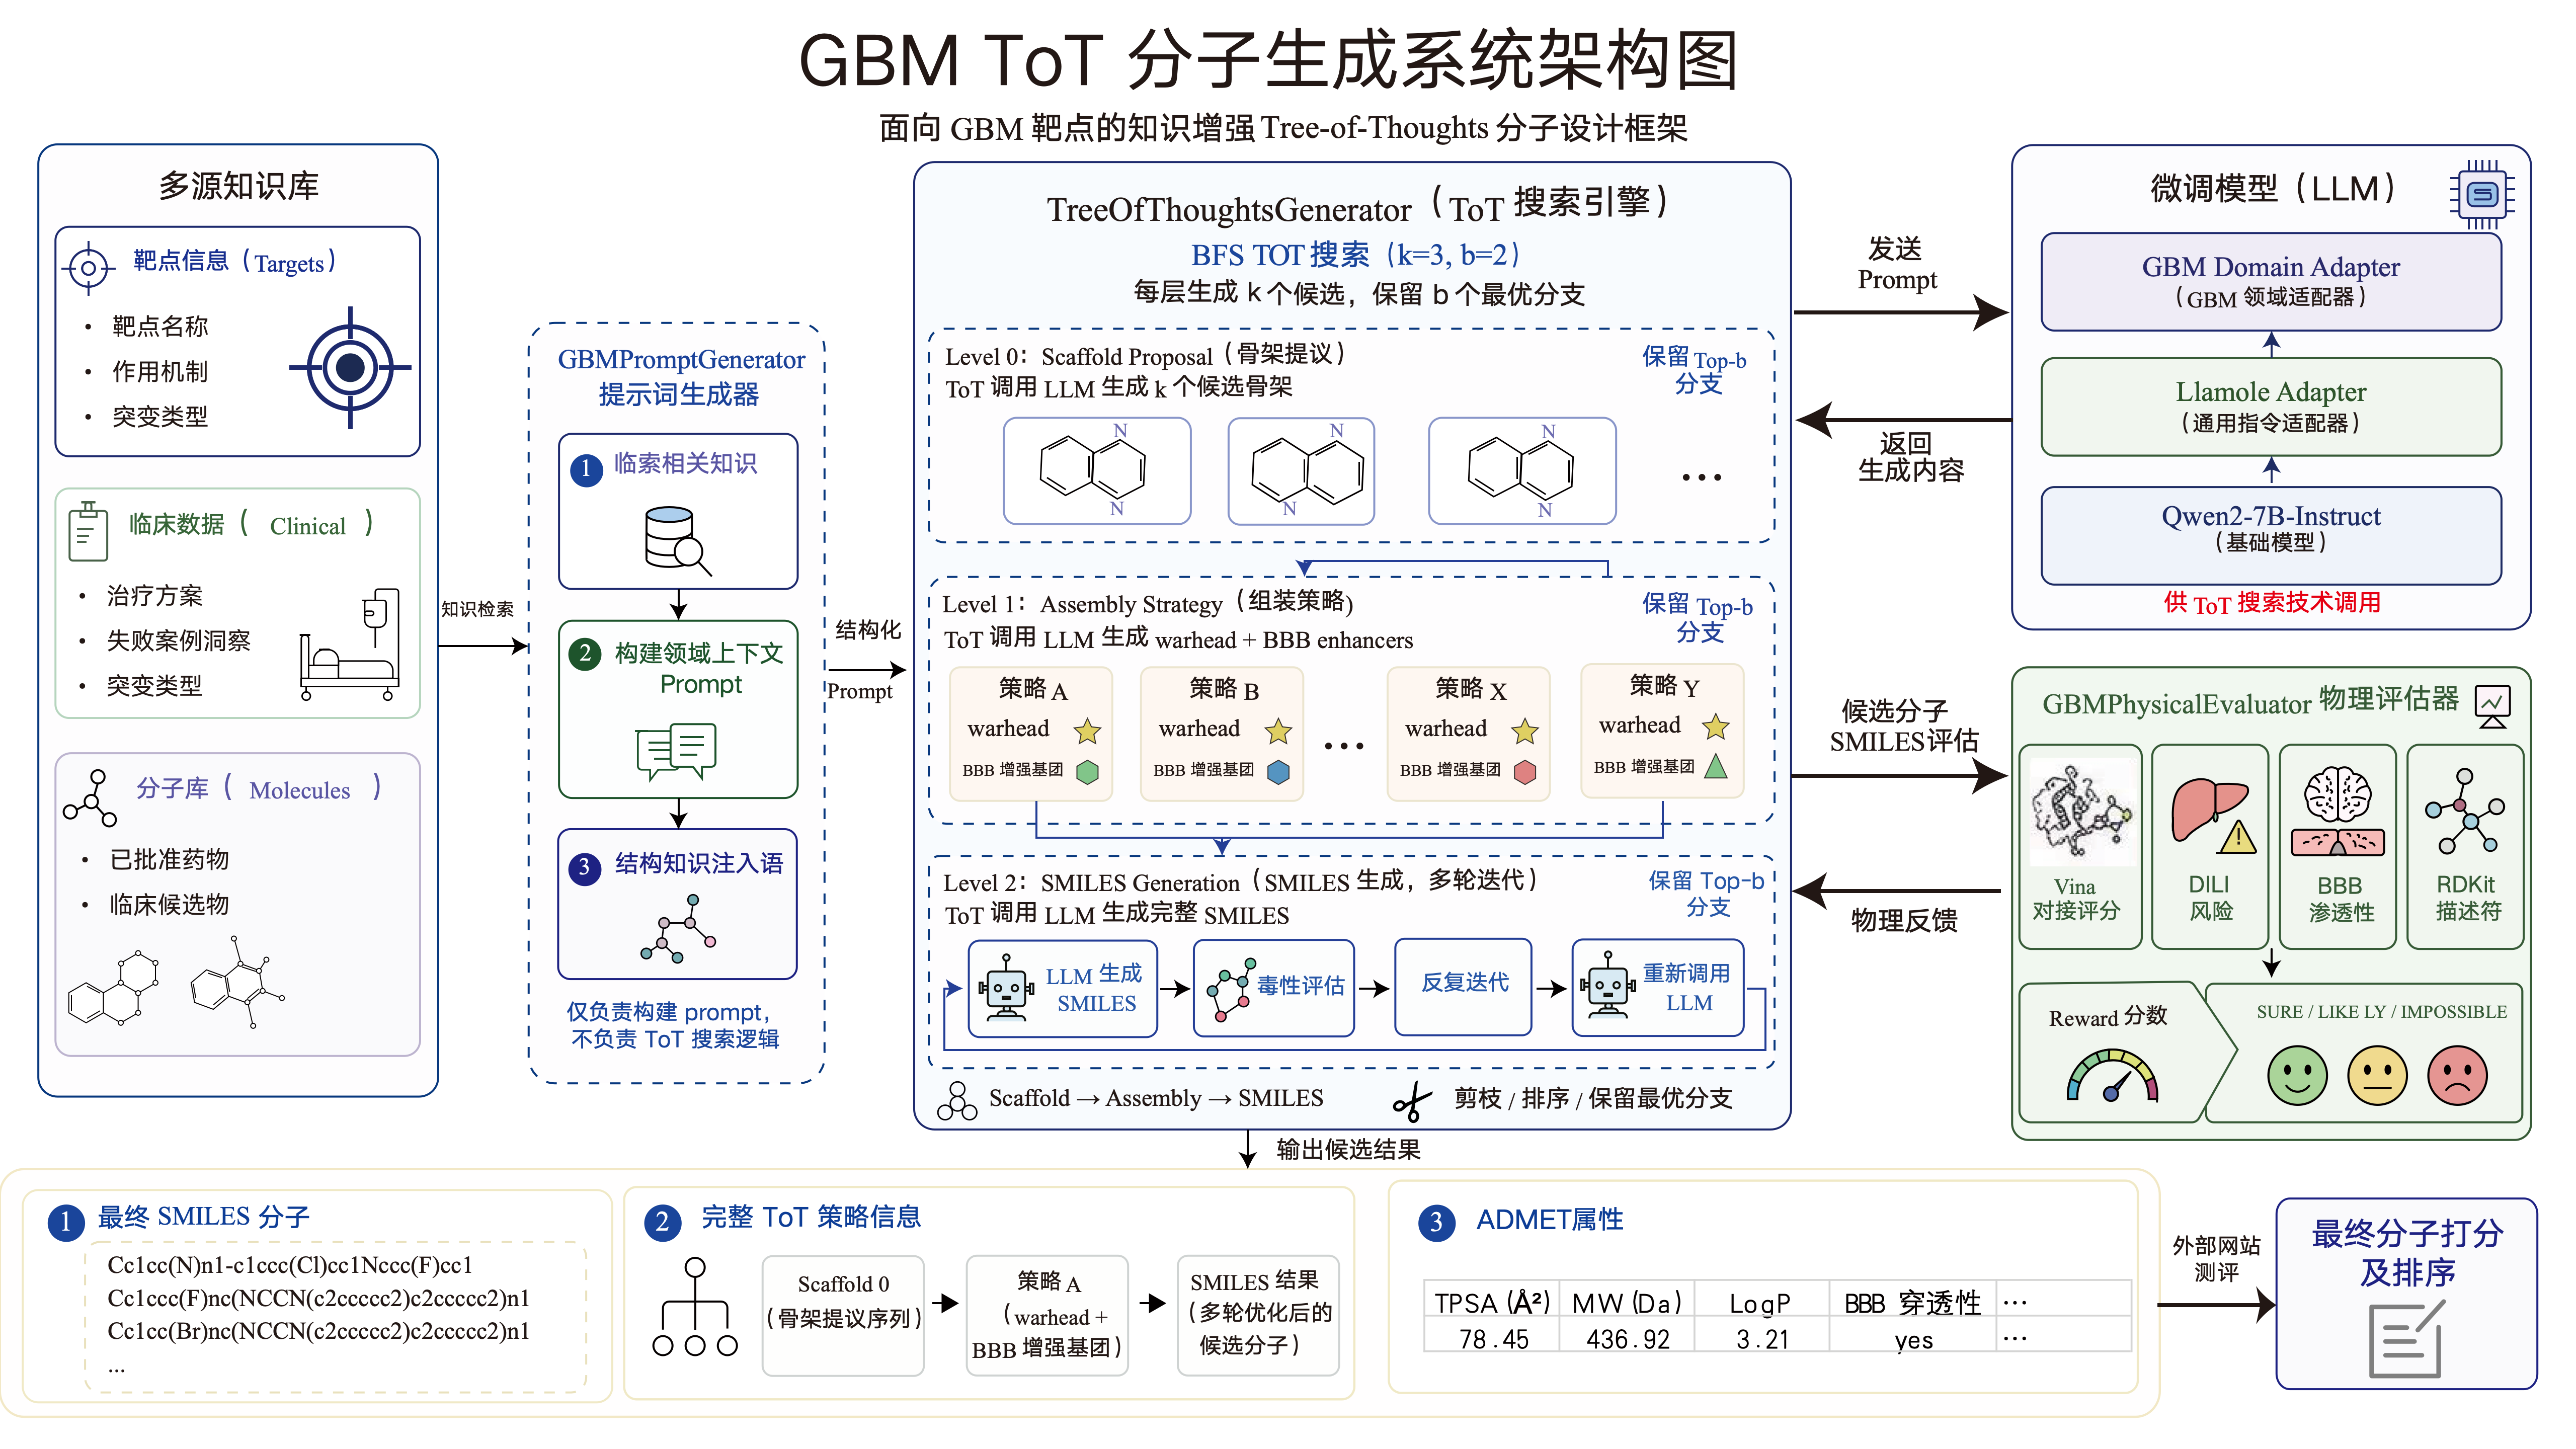
\includegraphics[width=0.9\textwidth]{图片/系统架构图.png}
    \caption{GBM候选分子生成系统架构图}\label{fig:system-arch}
\end{figure}

GBM候选分子生成涉及疾病靶点背景、CNS成药性约束和后续计算评价等多类信息，如果这些信息只在生成结束后统一筛选，容易造成大量候选结构在后续评估阶段被剔除。因此，本文在框架设计中将知识输入、结构生成和物理反馈三个环节前置到同一生成流程中，使候选分子在生成阶段就受到GBM任务条件的约束。

在输入端，系统接收目标靶点名称、生成分子数量上限以及配置需求。GBM领域知识库根据靶点名称返回相关靶点背景、CNS药物设计规则、参考分子结构和风险提示，Prompt生成器再将这些信息组织为模型可读取的任务输入。在生成端，Llamole负责完成文本条件到分子图结构的映射，CoT-ToT策略则进一步将候选分子设计过程拆分为骨架提议、片段组装和SMILES生成三个阶段。生成得到的候选结构随后进入物理评估模块，接受SMILES解析、理化性质检查、BBB经验评分、Vina对接和结构风险检测，这一模块的评价结果用于生成阶段的剪枝和反馈。

系统输出包括两个层次。第一层次是生成阶段输出，主要包括候选分子SMILES、分阶段推理结果以及对应的中间评价信息。第二层次是排序阶段输出，即经过外部工具重新计算和综合评分后的Top候选分子列表。通过这种设计，GBM-PharmaMind能够将疾病知识、多模态生成和计算评价组织为连续流程。

\section{GBM多模态知识库构建}\label{sec:knowledge-base}

\subsection{GBM领域知识库的构建必要性}

GBM候选分子生成对领域知识具有较强依赖。与一般分子生成任务相比，GBM任务不仅需要关注靶点结合潜力，还需要同时考虑BBB限制、CNS药物理化要求以及既有治疗经验。若仅向模型提供靶点名称，生成过程容易退化为通用化学空间中的结构采样，难以体现GBM任务的疾病特异性。因此，本文构建GBM多模态知识库，为后续Prompt生成、LoRA适配和物理评估提供统一的领域输入。该模块要求：知识库中的内容不仅用于背景说明，还需要能够转化为Prompt约束、LoRA适配数据和候选分子评价参考。

\subsection{ GBM 领域知识库构建与生成约束注入}

本文将知识库划分为GBM靶点信息库、GBM临床治疗数据库、GBM分子参考数据库和结构知识库四个部分。四类知识并不是相互独立的背景材料，而是在Prompt构建过程中共同提供靶点背景、临床约束、参考结构和分子设计规则。通过这种组织方式，模型在生成候选分子时不仅能够获得靶点名称，还能够同时接收与GBM疾病背景、CNS成药性要求和结构风险相关的约束信息。

GBM靶点信息库主要记录候选分子生成所需的疾病靶点背景。本文重点整理EGFR、VEGF/VEGFR和IDH1/IDH2等代表性靶点的信息。其中，EGFR是GBM中研究较成熟且突变频率较高的靶点，已有较多抑制剂结构和母核信息可作为生成参考\cite{Fu2025}；VEGF/VEGFR与肿瘤血管生成密切相关，但抗血管生成治疗在总体生存改善方面仍存在局限，因此相关候选分子生成需要考虑该靶点作用机制的复杂性\cite{Fu2025}；IDH1/IDH2与代谢重编程和分子分型相关，突变体口袋结构相对明确，适合用于对接评估和候选分子筛选\cite{Fu2025}。围绕这些靶点，知识库中记录靶点名称、相关分子亚型、突变或表达特征、已知抑制剂或药物、推荐分子量范围、推荐LogP范围、BBB相关要求以及设计风险提示等字段。

GBM临床治疗数据库用于补充疾病治疗背景和临床经验。标准治疗方案和TMZ耐药机制是理解GBM治疗现状的重要基础\cite{Stupp2005}，而BBB限制则是CNS药物设计中必须前置考虑的核心约束\cite{Pardridge2012}。这些信息进入Prompt后，可以帮助模型避免仅围绕靶点结合活性生成分子，而忽略脑部递送和治疗背景。与此同时，部分失败临床试验所反映的问题也可作为风险提示，用于减少重复已知低效策略的可能性\cite{Fu2025}。

GBM分子参考数据库主要保存已获批药物、临床试验分子以及相关候选结构的信息。本文将替莫唑胺等已知CNS药物结构作为参考，使模型能够学习已有药物的结构特点\cite{Stupp2005}；同时，临床试验分子的骨架类型和设计原则也被纳入数据库，为后续骨架提议和片段组装提供结构参照\cite{Fu2025}。结构知识库则进一步补充药物化学层面的规则信息，包括BBB优化基团、PAINS警告结构和Lipinski五规则等内容。BBB优化基团如烷氧基取代和氮杂环可为提高BBB穿透倾向提供设计参考\cite{Ferraris2020}；PAINS警告结构需要在生成阶段进行规避，以减少泛筛选干扰化合物的产生\cite{Baell2010}；Lipinski五规则则作为类药性判断的基础依据\cite{Pardridge2012}。

实际调用过程中，知识库先根据目标靶点名称检索对应的靶点背景和设计字段，再补充临床治疗经验、参考分子结构以及结构风险提示。系统通过结构化模板将上述信息写入Prompt，使靶点背景、BBB约束、结构风险和参考骨架能够在生成阶段共同参与分子设计。

该过程如算法\ref{alg:kb-prompt}所示。

\begin{algorithm}
\caption{基于知识库检索的Prompt构建算法}
\label{alg:kb-prompt}
\textbf{输入}：目标靶点名称$T$、知识库$K$、理化约束$C$ \\
\textbf{输出}：携带GBM领域知识的完整Prompt $P_T$

\begin{algorithmic}[1]
\Function{BuildKnowledgePrompt}{$T, K, C$}
    \State $\text{target\_info} \leftarrow \text{KB.get\_target\_info}(T)$    \Comment{从靶点信息库检索靶点背景}
    \State $\text{clinical\_insights} \leftarrow \text{KB.get\_clinical\_insights}()$    \Comment{从临床数据库检索治疗洞察}
    \State $\text{reference\_mols} \leftarrow \text{KB.get\_similar\_molecules}(T, \text{limit}=3)$    \Comment{从分子库检索参考骨架}
    \State $\text{structural\_guidance} \leftarrow \text{StructuralInjector.inject}(T)$    \Comment{从结构知识库注入骨架与BBB指导}
    \State $\text{bbb\_constraint} \leftarrow \text{FormatBBB}(\text{target\_info})$    \Comment{读取BBB约束字段（MW上限、TPSA上限）}
    \State $\text{risk\_warning} \leftarrow \text{FormatRisk}(\text{target\_info})$    \Comment{读取结构风险提示（如EGFRvIII变体风险）}
    \State $\text{template} \leftarrow \text{LoadPromptTemplate}(T)$    \Comment{加载靶点对应的Prompt模板}

    \State $P_T \leftarrow \text{template.format}($
        \Statex \hspace{1.2em} $\text{靶点背景}=\text{target\_info.description},$
        \Statex \hspace{1.2em} $\text{临床洞察}=\text{clinical\_insights},$
        \Statex \hspace{1.2em} $\text{参考骨架}=\text{reference\_mols},$
        \Statex \hspace{1.2em} $\text{结构指导}=\text{structural\_guidance},$
        \Statex \hspace{1.2em} $\text{BBB约束}=\text{bbb\_constraint},$
        \Statex \hspace{1.2em} $\text{风险提示}=\text{risk\_warning},$
        \Statex \hspace{1.2em} $\text{理化约束}=C$
    \State $)$
    \State \Return $P_T$
\EndFunction
\end{algorithmic}
\end{algorithm}

算法\ref{alg:kb-prompt}展示了知识库到Prompt的转换过程。目标靶点输入后，系统依次读取靶点信息、临床洞察、参考骨架和结构指导，并将BBB约束、风险提示和理化约束写入统一模板。通过该流程，分散的GBM领域知识被整理为生成模型可直接读取的结构化输入，从而为后续LoRA适配、CoT-ToT生成和物理评估反馈提供基础。

\section{Prompt生成器设计}\label{sec:prompt-generator}

\subsection{Prompt生成器的设计必要性}

LLM的输出质量高度依赖输入Prompt的设计~\cite{Wei2022,jin2025effective}。在分子生成任务中，Prompt需要包含以下要素：

\begin{itemize}
    \item \textbf{靶点背景}用于帮助LLM理解"EGFR"等靶点名称所对应的生物学含义~\cite{Fu2025}；
    \item \textbf{显式理化约束}用于增强模型对MW、LogP、TPSA等数值条件的遵循能力~\cite{Pardridge2012}；
    \item \textbf{风险结构约束}用于在生成阶段减少PAINS、DILI和hERG等潜在风险结构的出现~\cite{Aronov2008}；
    \item \textbf{CoT步骤}用于将复杂的分子设计任务拆分为可检查的中间过程~\cite{Wei2022}。
\end{itemize}

设目标靶点为$T$，知识库中与该靶点相关的领域信息为$K_T$，生成约束集合为$C$，推理格式约束为$H$，则Prompt生成器可表示为：
$$P_T = G(T, K_T, C, H)$$
其中，$G(\cdot)$表示Prompt生成函数。生成后的$P_T$同时包含靶点背景，理化性质范围、结构风险提示和输出格式要求，用于使不同靶点在统一约束体系下进入生成流程。

\subsection{Prompt生成器的核心方法}

具体而言，\texttt{generate\_full\_prompt()}负责构建完整任务输入；\texttt{build\_tot\_propose\_prompt()}负责生成骨架提议、片段组装和SMILES输出三个阶段的ToT提示；\texttt{build\_feedback\_injected\_prompt()}则用于将上一轮物理评估结果写入后续Prompt，使后续生成过程能够接收来自外部评估模块的反馈信息。

\section{分子图—文本协同生成模块}\label{sec:llamole-arch}

在GBM-PharmaMind中，Llamole承担从文本条件到分子结构的跨模态映射任务。设输入Prompt为$P_T$，语言模型首先得到隐层语义表示$h_T$，随后通过语义查询Token将该表示映射到图生成条件空间：
$$z_T = \phi(h_T)$$
其中，$\phi(\cdot)$表示图-LM连接器。图扩散模块在条件$z_T$的引导下生成候选分子图，并进一步转换为SMILES字符串。通过该过程，GBM靶点描述、BBB约束和结构风险提示能够以文本条件的形式参与分子图生成。本文不改变Llamole主体结构，而是在输入侧引入GBM知识约束，在适配侧加入LoRA，在输出侧连接物理评估反馈。

Llamole适合作为本文底层生成模型，主要原因在于其同时包含语言理解和分子图生成两部分能力。基础语言模型采用Qwen2-7B-Instruct\cite{Qwen2Team2024}，负责理解结构化分子设计任务中的靶点描述、约束条件和生成要求。为了使语言模型能够识别分子设计任务的边界，Llamole引入了特殊触发Token机制\cite{liu2025multimodal}。其中，\texttt{<design\_start>}和\texttt{<design\_end>}用于标记分子设计会话的起止，\texttt{<design\_body>}用于标记分子设计的具体内容，\texttt{<molecule>}用于标记分子结构输出位置。这些Token使模型能够在一般文本生成和分子生成任务之间建立明确边界，从而减少任务格式混淆。

在文本语义向分子图生成条件转换的过程中，语义查询Token承担中间桥接作用。模型从LLM隐层中提取与GBM任务相关的语义信息，例如高BBB穿透倾向、靶点结合需求和结构风险规避等内容，再通过线性投影层将其映射到图扩散模型可以使用的条件空间\cite{liu2025multimodal}。这一过程对应LLM语义空间到图模型条件空间的转换，也是Llamole能够将自然语言设计约束转化为分子图生成条件的关键步骤。

图-LM连接器用于完成语言模型与图生成模块之间的双向连接。其中，\texttt{lm\_to\_graph\_decoder}负责将LLM隐状态映射到图扩散解码器的条件空间，\texttt{graph\_to\_lm\_connector}用于将GNN编码得到的分子表示映射回LLM语义空间，\texttt{lm\_to\_graph\_predictor}则连接LLM与GNN预测器\cite{liu2025multimodal}。在候选分子生成过程中，模型首先接收由GBM知识库和Prompt生成器构建的任务输入，随后通过触发Token识别分子生成任务，并从隐层状态中提取语义查询向量。该向量经过图-LM连接器映射后，作为条件输入传递给图扩散模块，图扩散模块逐步生成候选分子图，最后由RDKit或图转换模块得到SMILES字符串。

上述流程如算法\ref{alg:llamole-gen}所示。

\begin{algorithm}
\caption{Llamole跨模态分子生成算法}
\label{alg:llamole-gen}
\textbf{输入}：GBM知识约束Prompt $P_T$ \
\textbf{输出}：候选分子SMILES字符串列表

\begin{algorithmic}[1]
\State $P_T \leftarrow \text{GBM知识约束Prompt}$    \Comment{来自知识库检索与Prompt生成器}

\State $\text{token\_ids} \leftarrow \text{tokenizer.encode}(P_T)$
\State $\text{inputs} \leftarrow \{\text{input\_ids}: \text{token\_ids}, \text{attention\_mask}: \text{ones}\}$

\State $\text{trigger\_id} \leftarrow \text{token\_id\_dict}[\texttt{<design\_start>}]$
\State $\text{inputs} \leftarrow \text{AddBodyTokens}(\text{inputs}, \texttt{<design\_body>}, \text{trigger\_id})$

\State $\text{lm\_outputs} \leftarrow \text{LanguageModel}(\text{inputs})$
\State $h_T \leftarrow \text{lm\_outputs.hidden\_states}[-1]$    \Comment{LLM最终隐层状态}

\State $\text{query\_vec} \leftarrow h_T[:, -N:\text{].mean(dim=1)}$    \Comment{提取最后N个Token的隐状态并平均，作为语义query向量}
\State $z_T \leftarrow \text{lm\_to\_graph\_decoder}(\text{query\_vec})$    \Comment{经线性投影层映射到图扩散条件空间}

\State $\text{mol\_graphs} \leftarrow \text{GraphDiffusionDecoder.generate}(\text{NONE}, z_T, \text{label\_idx})$    \Comment{图扩散模块在条件$z_T$引导下逐步去噪，生成候选分子图}
\State $\text{smiles\_list} \leftarrow [\text{RDKit.MolToSmiles}(\text{mol\_graph}) \text{ for } \text{mol\_graph} \text{ in } \text{mol\_graphs}]$    \Comment{图到SMILES转换}

\State \Return $\text{smiles\_list}$
\end{algorithmic}
\end{algorithm}

算法\ref{alg:llamole-gen}概括了Llamole从Prompt输入到SMILES输出的主要流程。GBM知识约束Prompt首先被编码为模型输入，语言模型生成隐层语义表示后，系统提取最后若干Token的隐状态作为语义query向量，并通过\texttt{lm\_to\_graph\_decoder}映射到图扩散条件空间。图扩散模块在该条件引导下生成候选分子图，最终转换为SMILES列表。由此可见，Llamole在本文框架中主要承担文本条件到分子结构的跨模态转换任务，而GBM-PharmaMind的改进重点在于输入侧的GBM知识约束、适配侧的LoRA领域调整以及输出侧的物理评估反馈。

\section{GBM领域LoRA适配}\label{sec:lora-finetune}

\begin{figure}[htbp]
    \centering
    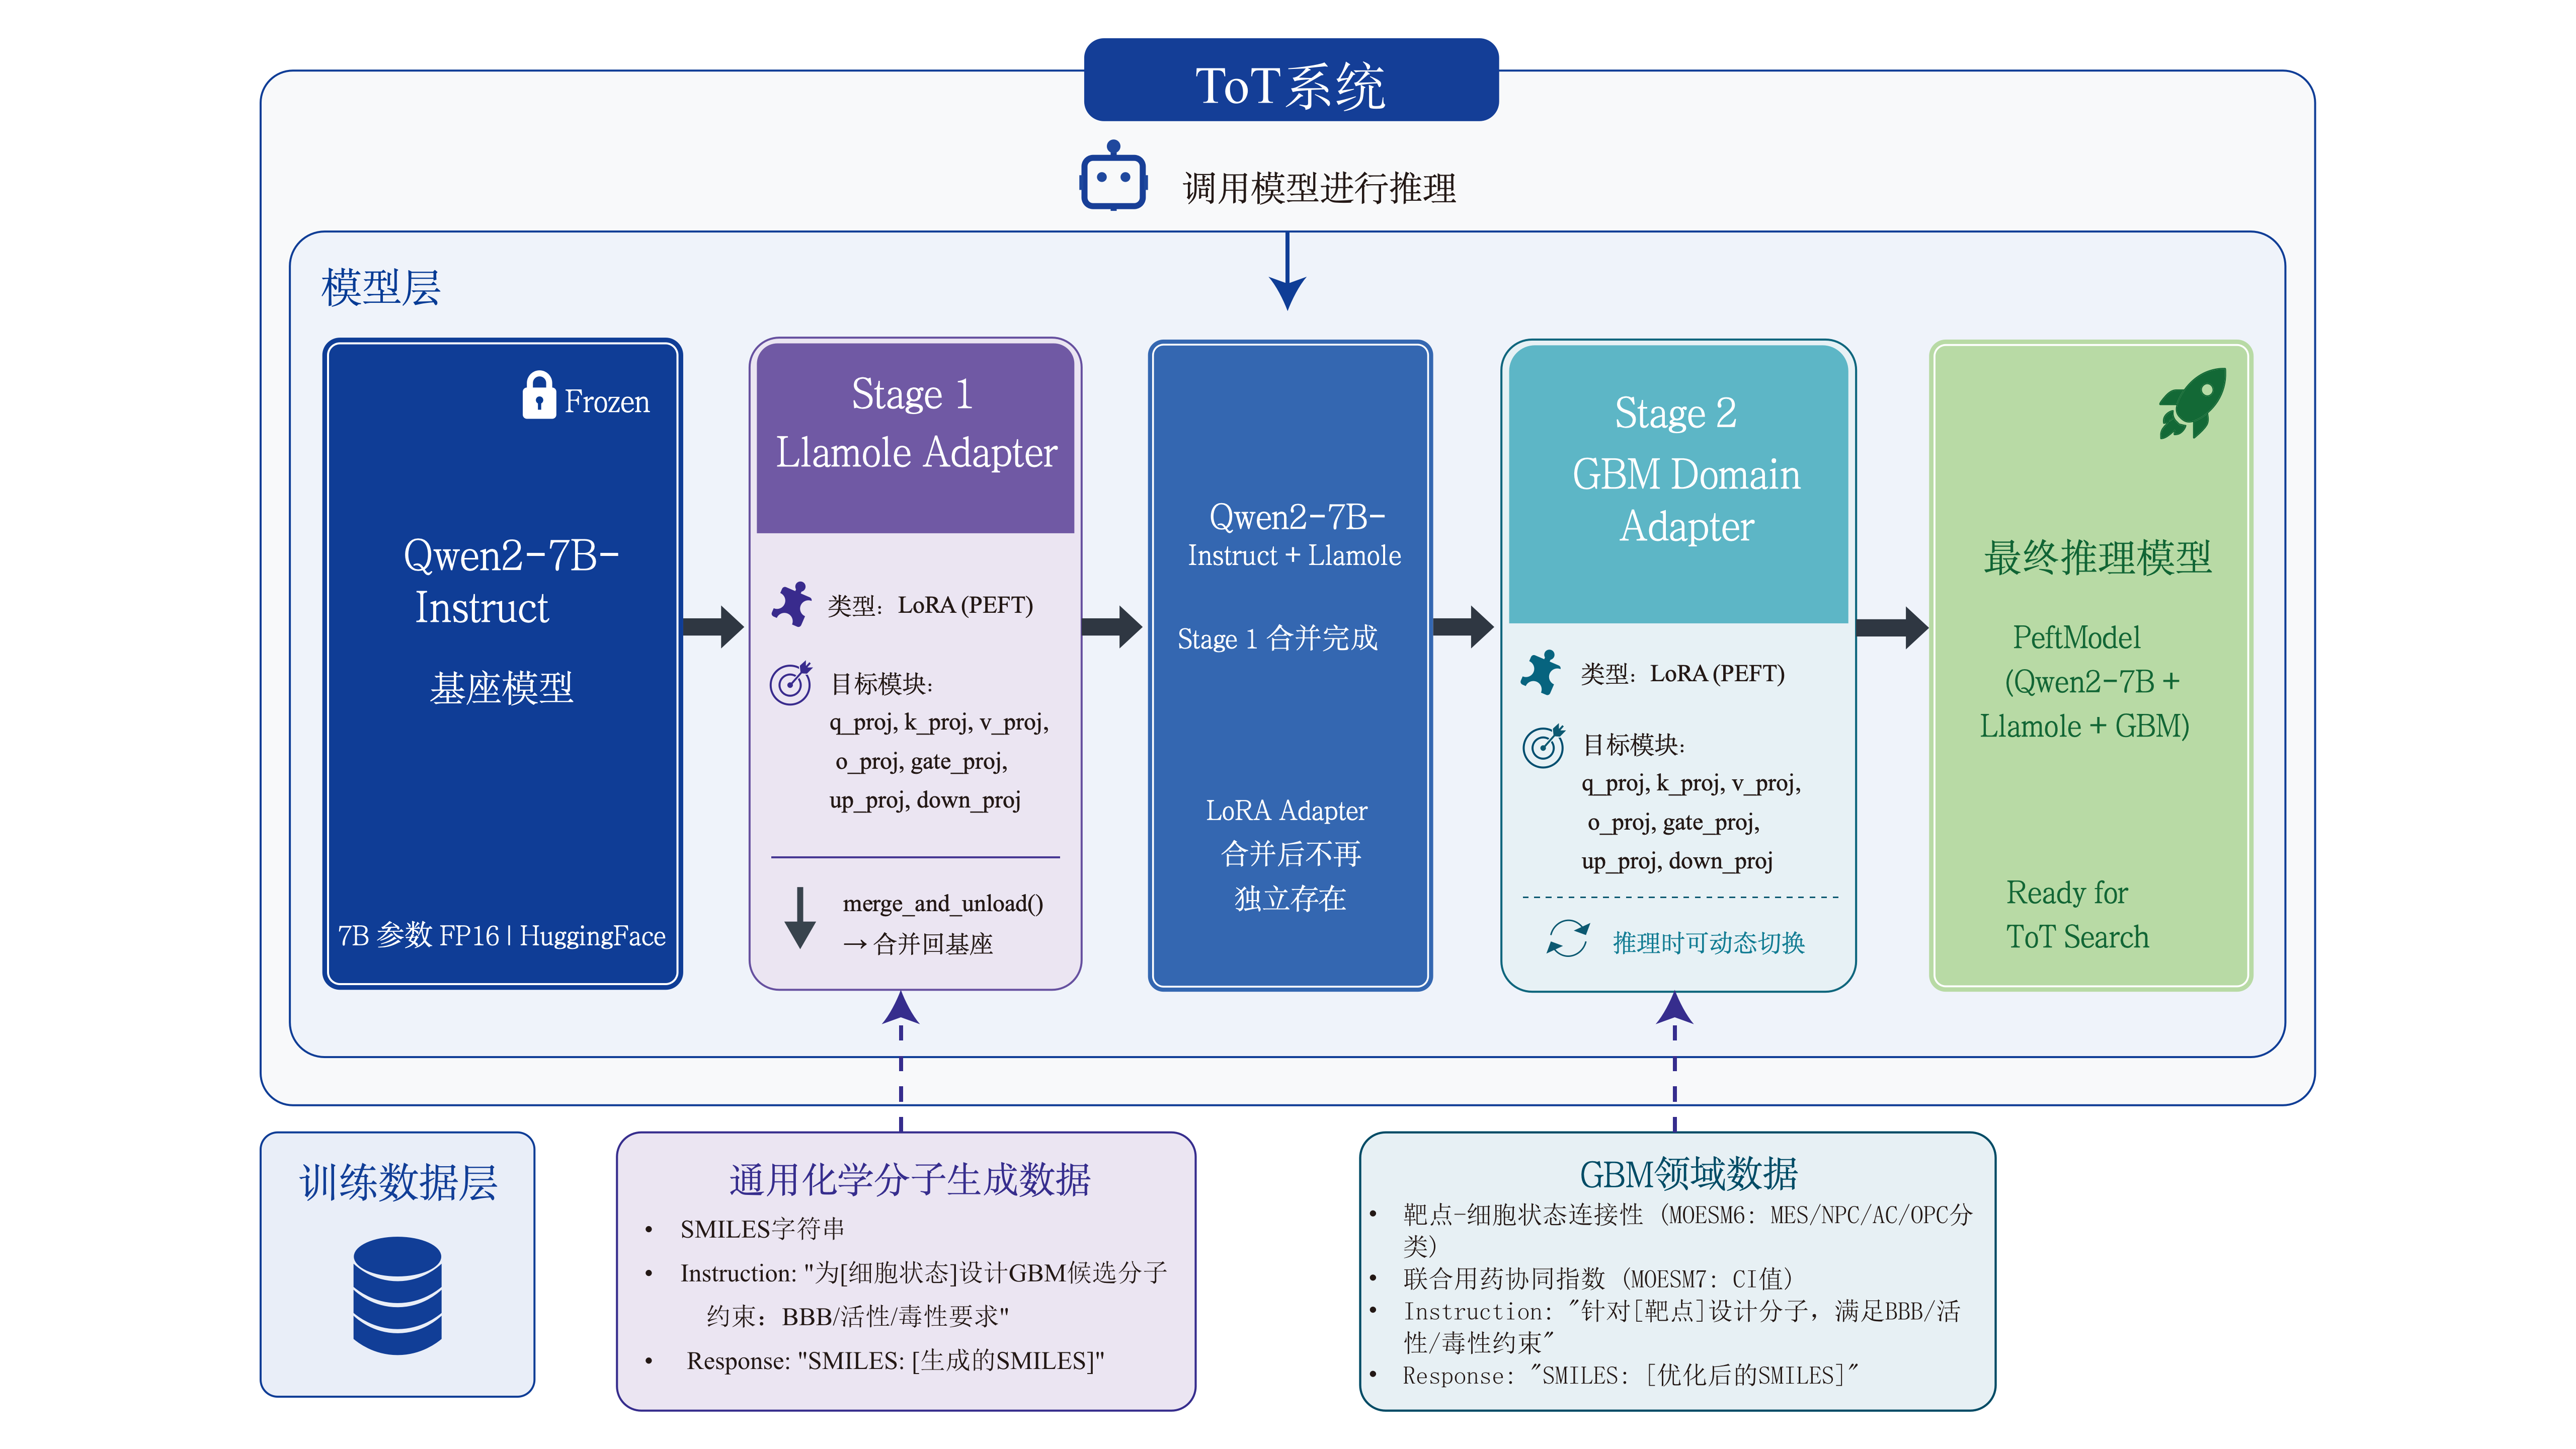
\includegraphics[width=0.9\textwidth]{图片/细节图3.png}
    \caption{GBM领域LoRA适配流程示意图}\label{fig:lora-flow}
\end{figure}

GBM领域LoRA适配可视为作用于基础语言模型参数空间的轻量化领域偏置层。设基础模型参数为$\Theta$，LoRA在目标线性层中引入低秩增量：
$$\Delta W = BA$$
其中，A和B为低秩矩阵，秩参数设置为16。模型实际推理时使用$W+\Delta W$进行计算。该设置使模型在保留原有语言理解能力的同时，引入GBM靶点描述、CNS理化约束和候选分子生成偏好的任务相关信息。本文采用两阶段适配流程：先在通用化学分子生成数据上完成Llamole Adapter适配，再基于GBM领域数据构建GBM Domain Adapter。$r=16$的设置用于在表示能力与训练开销之间取得折中。

LoRA的核心配置参数如表\ref{tab:lora-config}所示：

\begin{table}[htbp]
    \centering
    \caption{LoRA配置参数}\label{tab:lora-config}
    \begin{tabular}{ll}
        \toprule
        \textbf{参数} & \textbf{值} \\
        \midrule
        $r$ (秩) & 16 \\
        lora\_alpha & 32 \\
        lora\_dropout & 0.05 \\
        bias & none \\
        目标模块 & q\_proj, k\_proj, v\_proj, o\_proj, \\
                 & gate\_proj, up\_proj, down\_proj \\
        \bottomrule
    \end{tabular}
\end{table}

选择$r=16$的原因是在表示能力和训练参数之间取得平衡~\cite{hu2022lora}：$r$过小会限制LoRA的表示能力~\cite{hu2022lora}，$r$过大则增加训练开销~\cite{hu2022lora}。$r=16$意味着可训练参数量约为$16 \times (4096 \times 2) \approx 130$K（对于Qwen2-7B的注意力层），远小于全量微调~\cite{hu2022lora}。

\section{CoT-ToT协同生成算法}\label{sec:cot-tot-algorithm}

GBM候选分子生成并不是单一的字符串生成任务，而是同时受到靶点条件、BBB穿透倾向、毒性风险和基础理化性质约束的多阶段生成任务。若直接要求模型一次性输出完整SMILES，模型虽然可以给出形式上可解析的分子字符串，但其中的骨架选择、片段修饰和成药性考虑往往混杂在同一输出中，后续难以判断问题来自结构设计阶段还是来自SMILES表达阶段。因此，本文将CoT推理与ToT搜索结合，用于把候选分子生成过程拆分为更清晰的中间步骤。

本文框架中，CoT主要承担生成过程中的步骤组织作用。模型首先根据靶点背景和CNS药物设计要求，对候选分子的设计方向进行分解，明确骨架选择、局部修饰和最终结构表达之间的先后关系。ToT则用于在每个阶段保留多个候选方向，避免生成过程过早固定在单一结构路径上。两者结合后，模型不再只沿着一条线性推理链生成分子，而是可以在若干候选骨架和片段方案之间进行比较，并将物理评估结果用于后续分支调整。

本文将CoT-ToT生成过程划分为骨架提议、片段组装和SMILES生成三个阶段。骨架提议阶段主要确定候选分子的主体结构和可能的药效团方向，为后续局部修饰提供基础。片段组装阶段在已确定骨架的基础上引入取代基、连接片段或杂环结构，用于扩展候选分子的局部结构空间。SMILES生成阶段则将前两个阶段得到的结构设想转化为可解析的分子字符串，并交由RDKit和物理评估模块进行检查。这样的分阶段设计有助于将分子生成中的结构构思、局部优化和最终表达区分开来，也便于在生成过程中获取反馈信息。

ToT搜索宽度设置为3，主要考虑到候选分支数量与后续物理评估开销之间的平衡。若每一阶段保留过多分支，对接和性质计算的成本会明显增加；若分支数量过少，又容易降低结构探索的多样性。最大深度设置为2，对应骨架、片段和SMILES三个层级。图3.3展示了基于BFS的三阶段搜索流程，模型先生成候选骨架，再围绕保留骨架进行片段组装，最后输出SMILES并进入物理评估。评估结果会被重新写入下一轮Prompt，用于调整后续生成方向，从而形成生成、评估、反馈和再生成的循环。

\begin{figure}[H]
    \centering
    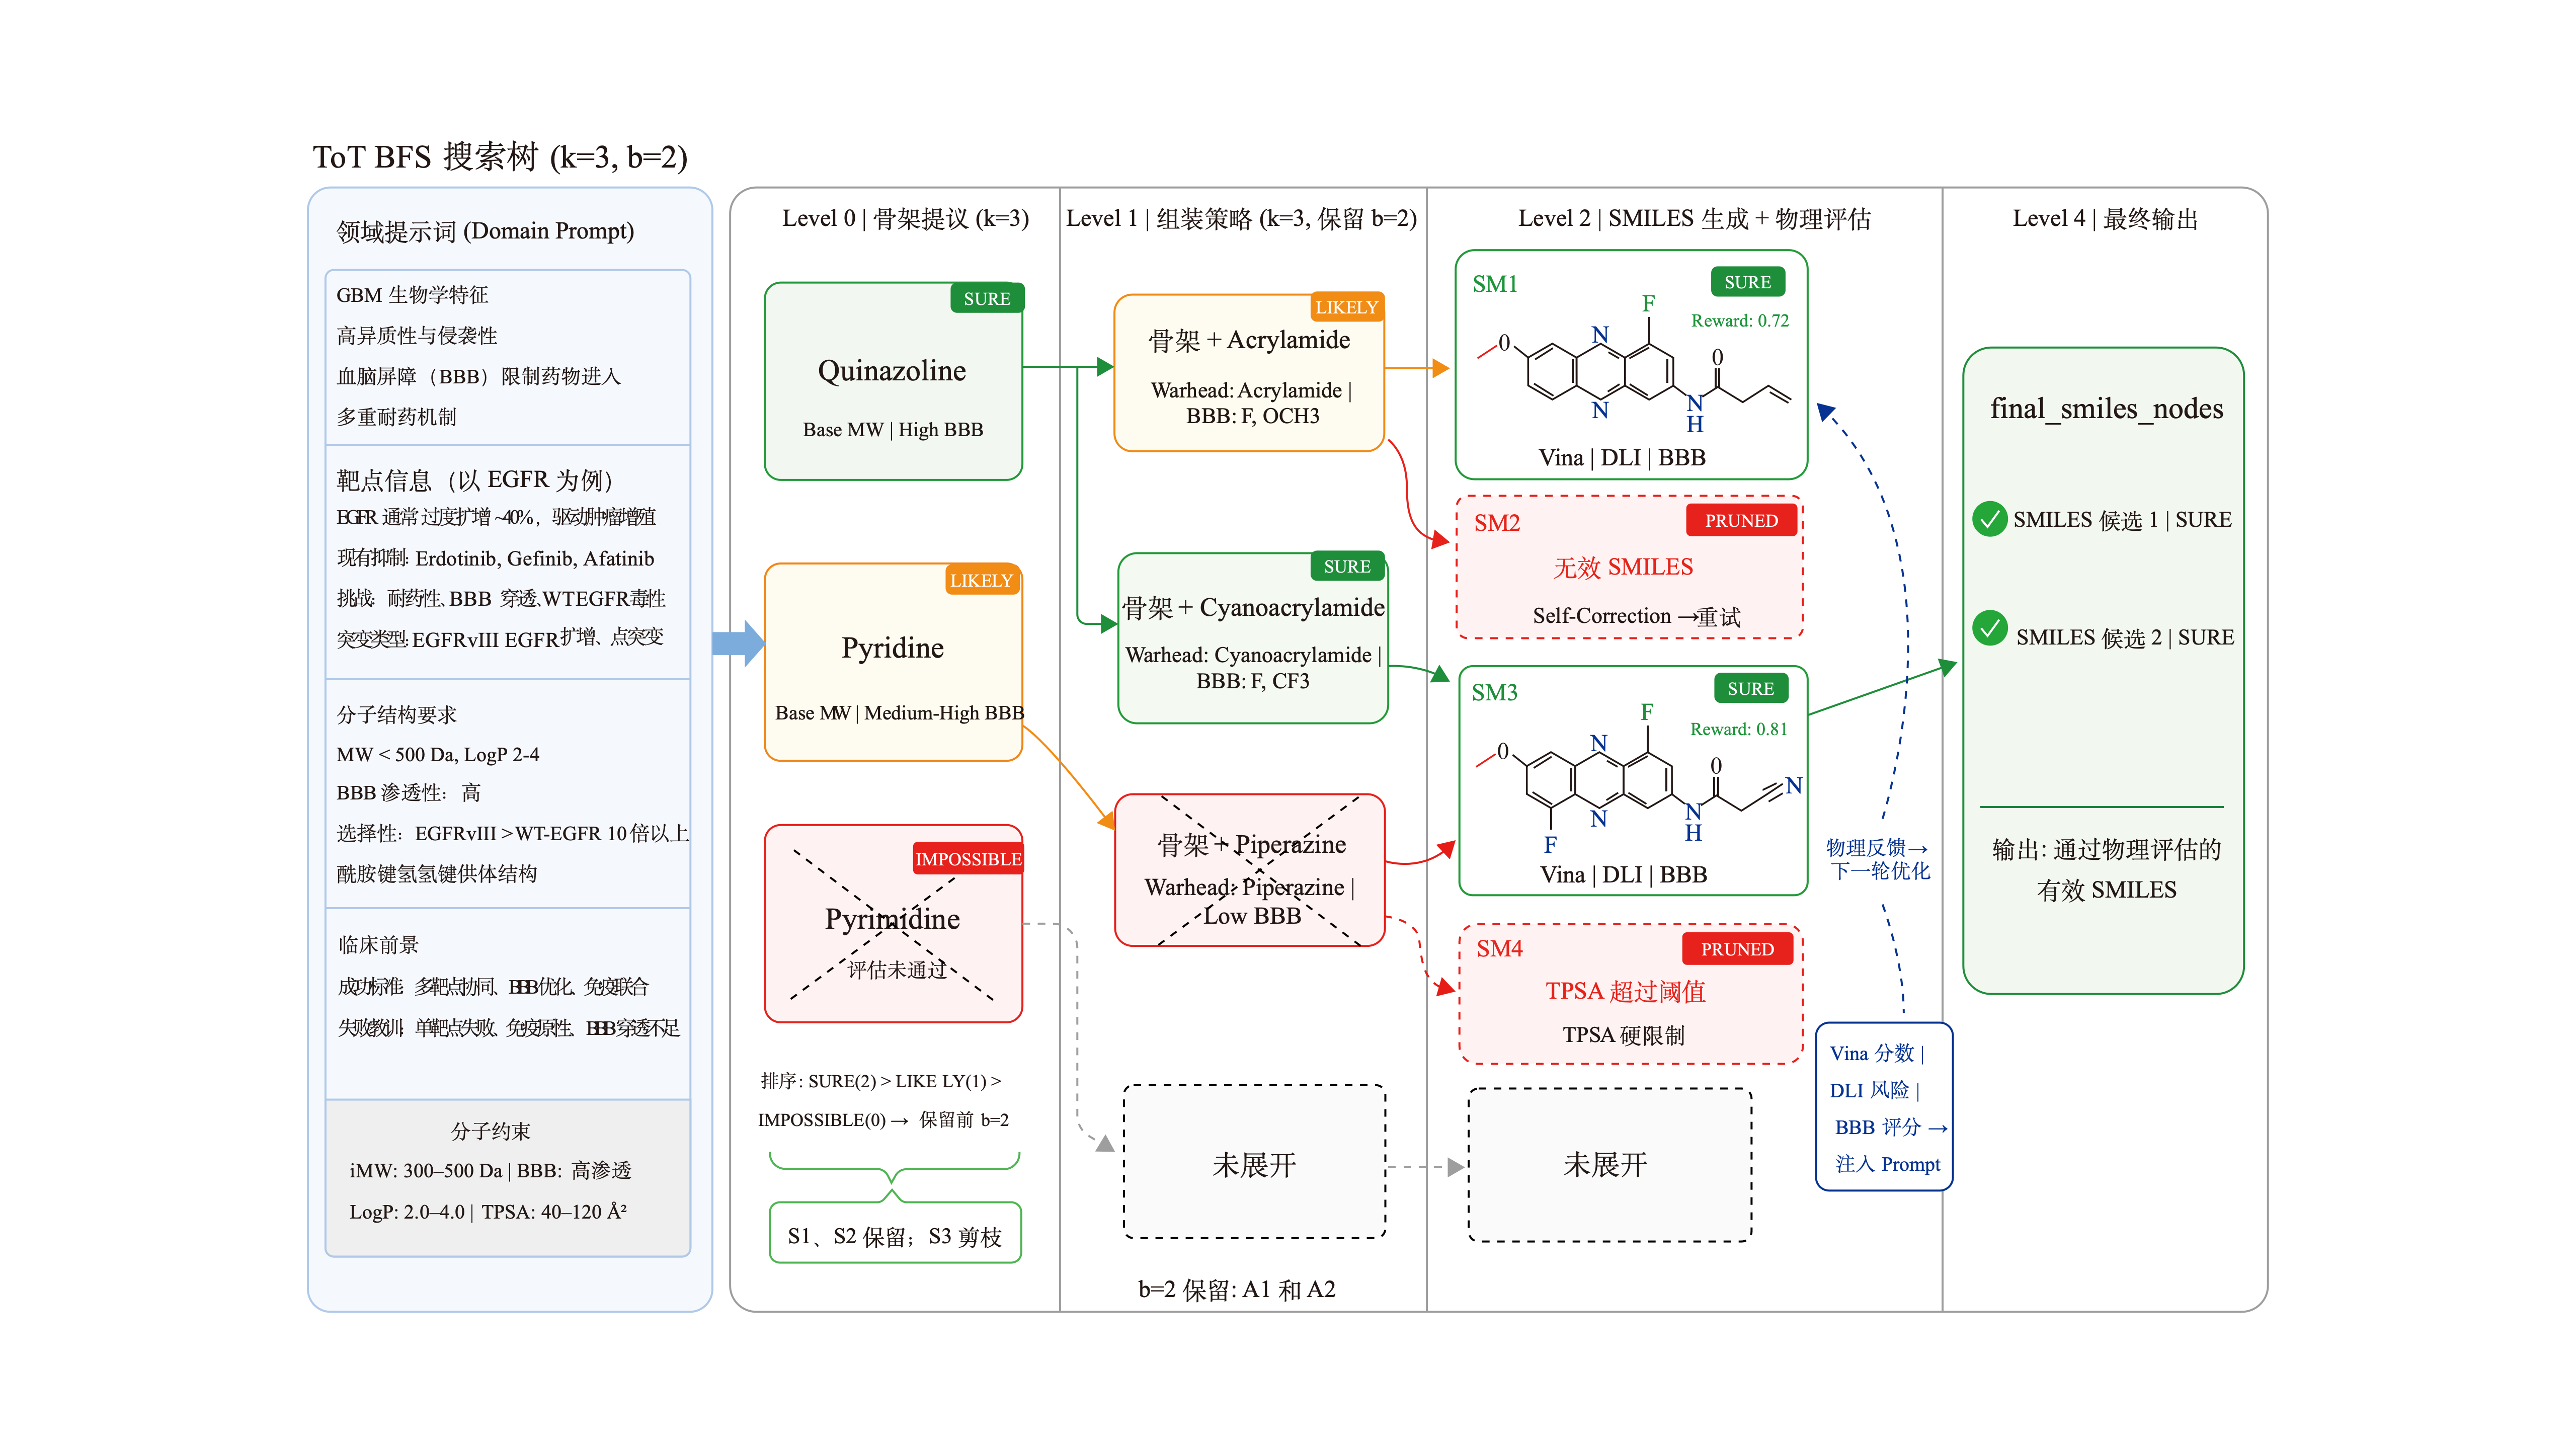
\includegraphics[width=0.9\textwidth]{图片/细节图2.png}
    \caption{基于ToT BFS搜索的三阶段候选分子生成流程示意图}\label{fig:tot-flow}
\end{figure}

该算法的核心伪代码如算法\ref{alg:cot-tot}所示。

\begin{algorithm}
\caption{基于CoT-ToT与物理反馈的GBM候选分子生成算法}
\label{alg:cot-tot}
\textbf{输入}：目标靶点$T$、生成数量上限$N$、知识库$K$、理化约束$C$、搜索宽度$k$、最大深度$d$ \\
\textbf{输出}：候选分子集合$M$及其评分集合$S$

\begin{algorithmic}[1]
\State \textbf{Step 1: 知识检索} \Comment{从知识库中获取靶点相关信息}
\State $K_T \leftarrow \text{QueryTargetKB}(K, T)$
\State $P_{CoT} \leftarrow \text{BuildCoTPrompt}(K_T, C)$ \Comment{构造CoT推理Prompt}

\State \textbf{Step 2: CoT推理} \Comment{使用CoT分解分子设计任务}
\State $R_{CoT} \leftarrow \text{MolecularLLM}(P_{CoT})$ \Comment{获取结构化推理结果}

\State $M \leftarrow \emptyset, S \leftarrow \emptyset$
\State $iter \leftarrow 0$

\While{$|M| < N$ and $iter < MAX\_ITER$}
    \State \textbf{Step 3: 骨架提议（ToT深度0）}
    \State $P_{scaffold} \leftarrow \text{BuildScaffoldPrompt}(R_{CoT}, K_T, C)$
    \State $S_{candidates} \leftarrow \text{MolecularLLM}(P_{scaffold})$ \Comment{生成$k$个候选骨架}
    \State $S_{valid} \leftarrow \text{FilterByBBB}(S_{candidates})$ \Comment{BBB约束预过滤}
    \For{$i \leftarrow 1$ \textbf{to} $|S_{valid}|$}
        \State $scaffold \leftarrow S_{valid}[i]$
        \State \textbf{Step 4: 片段组装（ToT深度1）}
        \State $P_{assembly} \leftarrow \text{BuildAssemblyPrompt}(scaffold, R_{CoT}, C)$
        \State $F_{candidates} \leftarrow \text{MolecularLLM}(P_{assembly})$ \Comment{生成$k$个片段方案}
        \For{$j \leftarrow 1$ \textbf{to} $|F_{candidates}|$}
            \State $fragment \leftarrow F_{candidates}[j]$
            \State \textbf{Step 5: SMILES生成（ToT深度2）}
            \State $P_{smiles} \leftarrow \text{BuildSMILESPrompt}(scaffold, fragment, C)$
            \State $SMILES \leftarrow \text{MolecularLLM}(P_{smiles})$
            \State \textbf{Step 6: SMILES解析与有效性验证}
            \State $mol \leftarrow \text{RDKitParse}(SMILES)$
            \If{$mol \neq \text{None}$ and $\text{IsValidPhysChem}(mol, C)$}
                \State \Comment{Step 7-11: 物理评估管线（生成阶段剪枝反馈）}
                \State $vina \leftarrow \text{VinaDock}(mol, T)$ \Comment{对接分数用于剪枝反馈}
                \State $bbb \leftarrow \text{BBBScore}(mol)$ \Comment{BBB评分用于剪枝反馈}
                \State $dili, herg \leftarrow \text{AlertCheck}(mol)$ \Comment{风险警报用于排除}
                \State $mp \leftarrow \text{MPOReward}(vina, bbb, dili, herg)$ \Comment{中间反馈评分}
                \State $score \leftarrow (vina, bbb, dili, herg, mp)$

                \State \Comment{Step 12: 硬截断与Delta Scoring}
                \If{$\text{HardFilter}(score)$}
                    \State \textbf{continue} \Comment{不合格分子被剪枝}
                \ElsIf{$\text{DeltaCheck}(score, iter) \leq 0.05$}
                    \State \Comment{Delta Scoring豁免：毒性增量不大于0.05时保留}
                \EndIf

                \State $M \leftarrow M \cup \{mol\}$
                \State $S \leftarrow S \cup \{score\}$

                \State \Comment{Step 13: 反馈注入}
                \State $P_{feedback} \leftarrow \text{BuildFeedbackPrompt}(score, R_{CoT})$
                \State $R_{CoT} \leftarrow \text{UpdateCoT}(R_{CoT}, P_{feedback})$
            \EndIf
        \EndFor
    \EndFor
    \State $iter \leftarrow iter + 1$
\EndWhile

\State \textbf{Step 14: Top-$K$排序与输出（基于 TotalScore 的最终排序）}
\State $(M_{sorted}, S_{sorted}) \leftarrow \text{RankByTotalScore}(M, S)$
\State \Return $(M_{sorted}[0:K], S_{sorted}[0:K])$
\end{algorithmic}
\end{algorithm}

该算法实现了"生成—评估—反馈—再生成"的循环：每轮生成后，SMILES生成阶段产生的分子经过物理评估管线打分，反馈结果通过Prompt注入下一轮CoT推理~\cite{Yao2023}，引导模型在下一轮生成时避免低评分分子特征~\cite{Yao2023}。

ToT搜索的三阶段（骨架提议、片段组装和SMILES生成）使得搜索空间逐步聚焦~\cite{Yao2023}：在骨架阶段探索宏观结构（3个分支）~\cite{Yao2023}，在片段阶段探索中观策略（3×3个分支）~\cite{Yao2023}，在SMILES阶段聚焦到具体分子~\cite{Yao2023}。在完成SMILES生成后，系统调用物理评估管线对分子进行打分，评估结果反馈至下一轮CoT推理用于指导改进~\cite{Yao2023}。这种分层搜索策略在探索广度和深度之间取得了平衡~\cite{Yao2023}。

\section{物理评估与闭环反馈}\label{sec:physics-evaluation}

\subsection{物理评估模块的作用}

物理评估模块通过外部工具对生成分子进行多维度量化评价，为候选结构的过滤、剪枝和反馈注入提供依据。该模块接收生成得到的SMILES字符串，并依次计算基础理化描述符、结构风险警报、BBB经验评分、Vina对接分数和MPO Reward，最终形成可用于后续Prompt反馈的评估结果。消融实验结果表明，去除物理评估后DrugCLIP均值下降24.0\%，说明该模块对生成质量具有一定贡献。

为避免生成阶段反馈与最终候选排序在功能上混同，本文将评价指标划分为过程性指标和终局性指标。过程性指标参与生成循环中的过滤、剪枝和反馈注入，终局性指标用于生成结束后的候选分子优先级排序。过程性评价集合可记为：
$$E_g = \{S_{\text{vina}}, S_{\text{BBB}}, A_{\text{DILI}}, A_{\text{hERG}}, R_{\text{MPO}}\}$$
其中，$S_{\text{vina}}$和$S_{\text{BBB}}$分别表示Vina对接分数和BBB经验评分，$A_{\text{DILI}}$与$A_{\text{hERG}}$表示结构风险警报，$R_{\text{MPO}}$表示生成阶段综合反馈得分。终局性指标由TotalScore表示，用于对通过基本过滤的候选分子进行统一排序。

\begin{figure}[htbp]
    \centering
    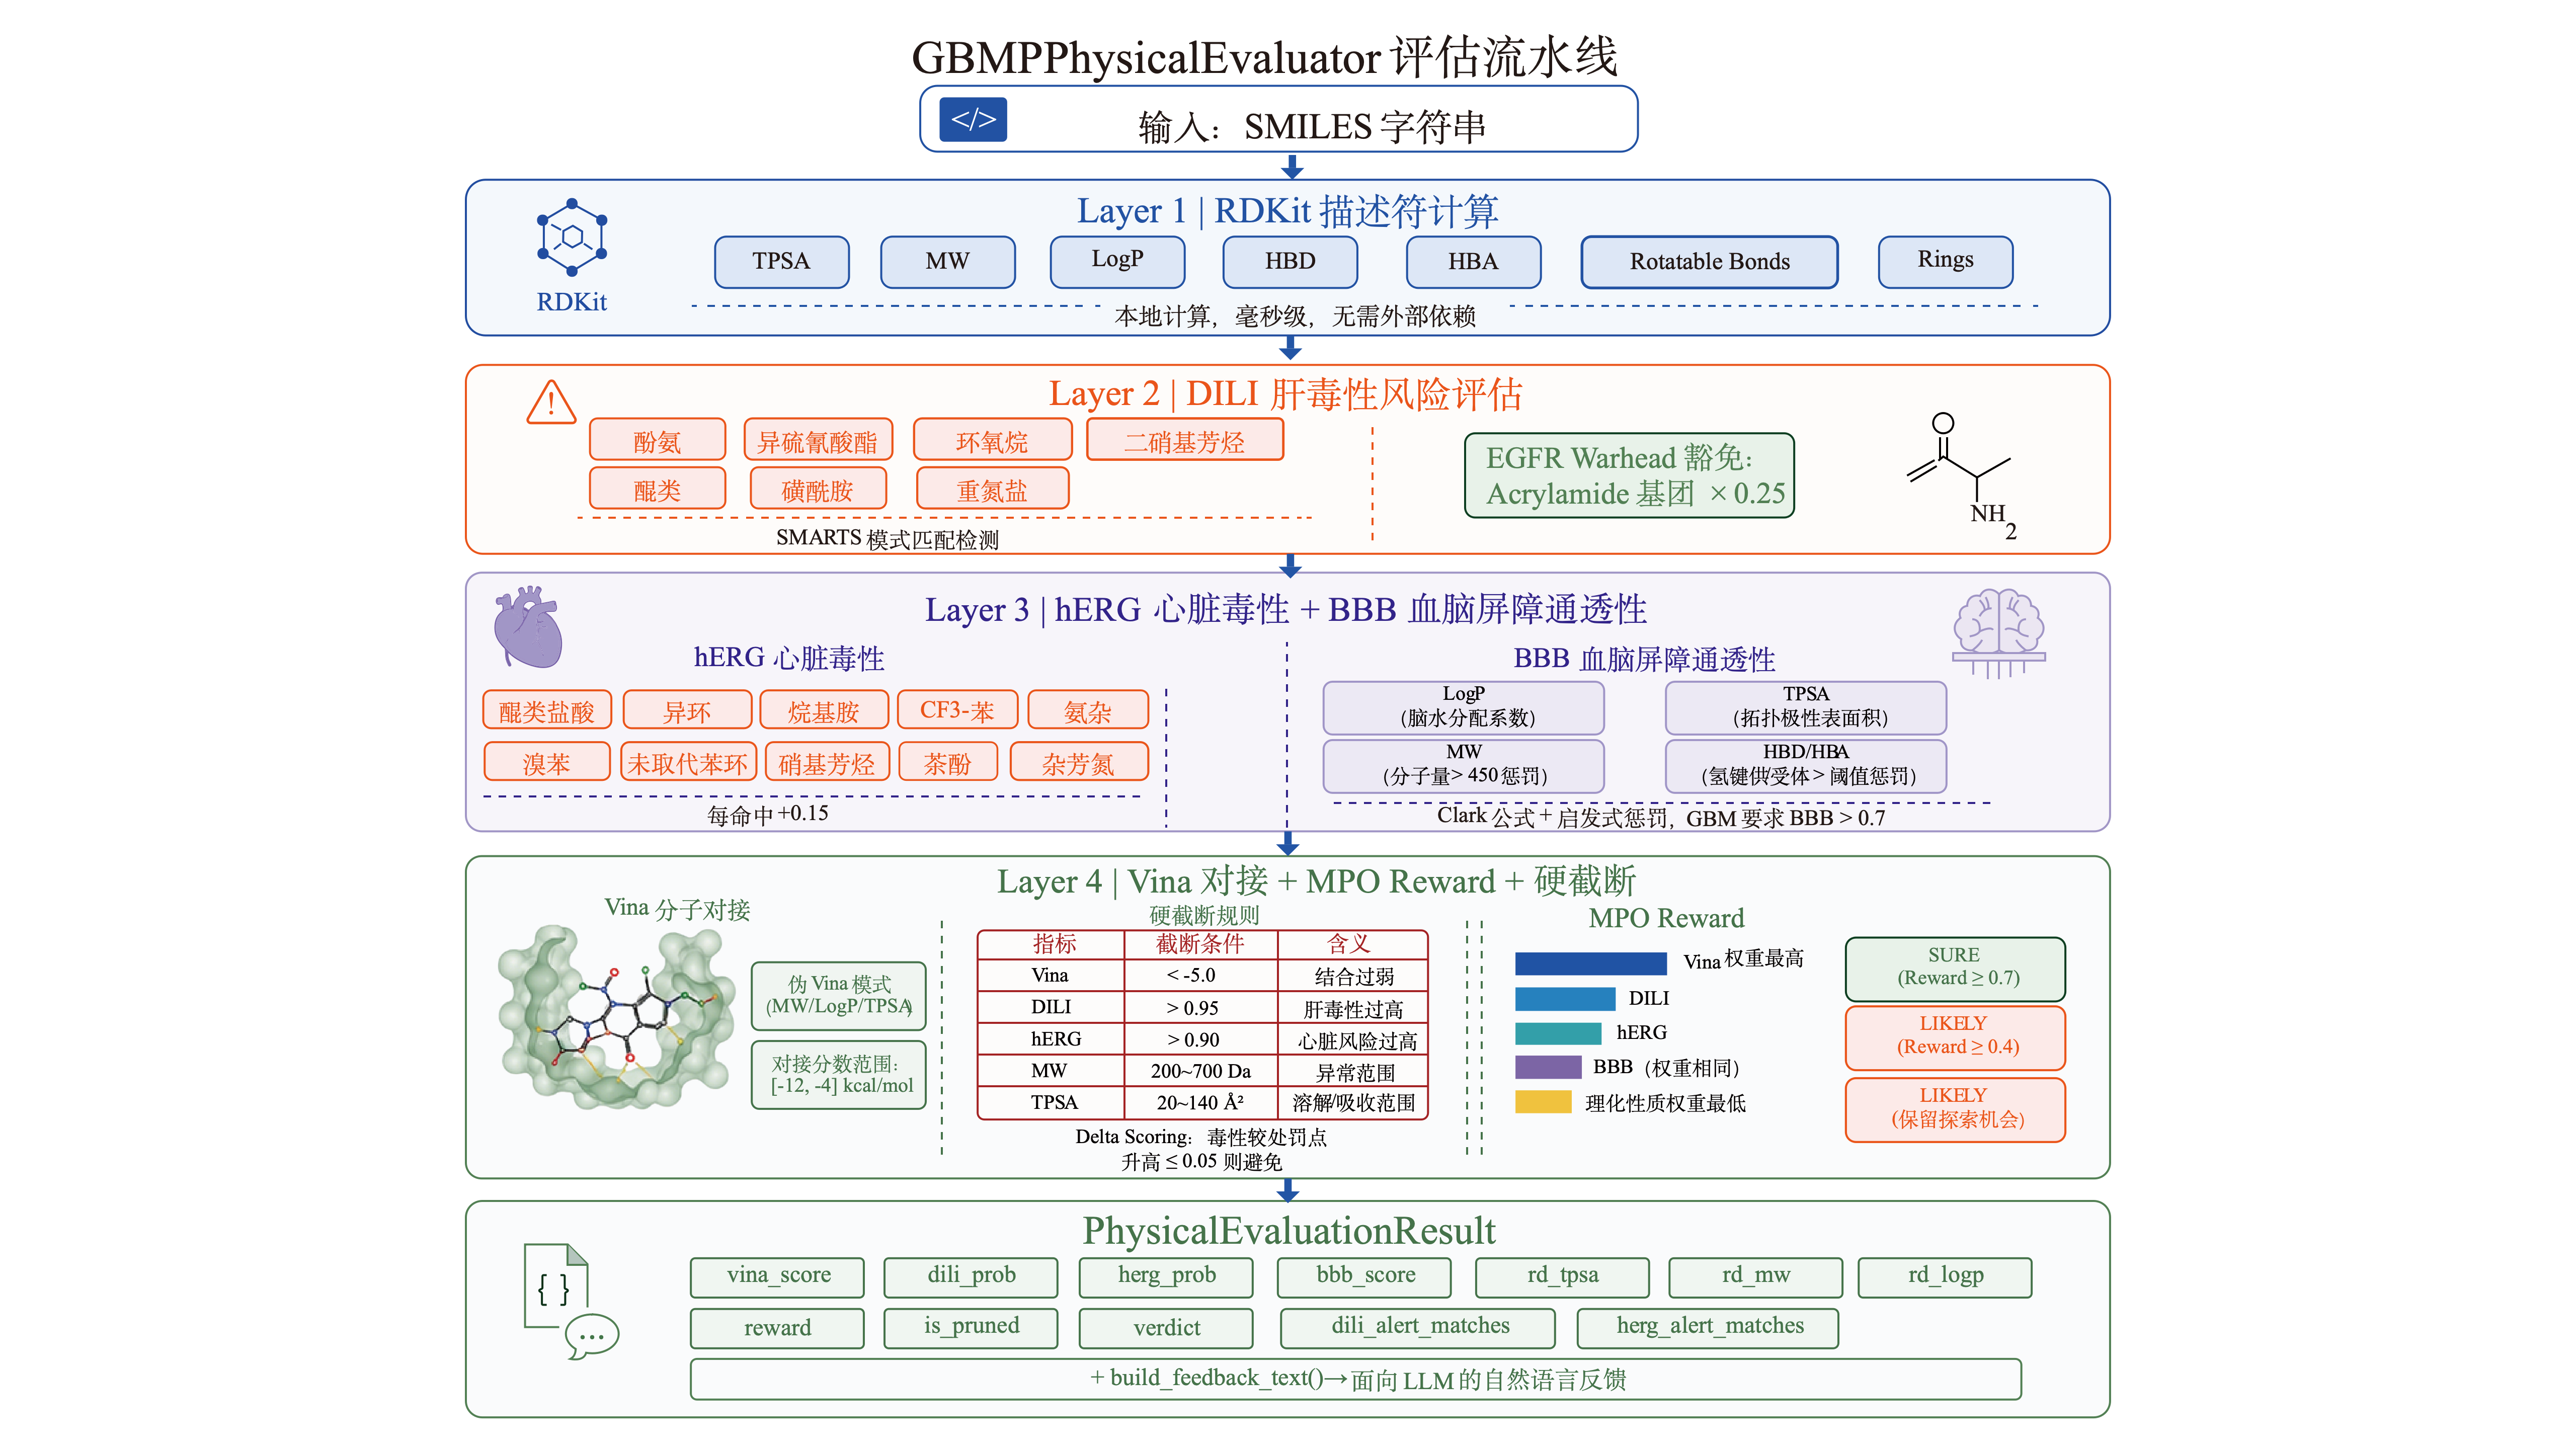
\includegraphics[width=0.9\textwidth]{图片/细节图1.png}
    \caption{GBMPPhysicalEvaluator物理评估流水线示意图}\label{fig:physics-arch}
\end{figure}

\subsection{AutoDock Vina对接}

AutoDock Vina~\cite{Trott2010}用于计算生成分子与靶点蛋白的对接亲和力（kcal/mol）。Vina分数的评估标准为：

\begin{itemize}
    \item Vina < -7.0 kcal/mol：对接分数处于较优区间（强结合参考阈值~\cite{Trott2010}）
    \item -7.0 ≤ Vina < -5.0 kcal/mol：中等结合
    \item Vina ≥ -5.0 kcal/mol：弱结合，触发硬截断剪枝
\end{itemize}

Vina分数在本文中的定位是"生成阶段剪枝反馈"~\cite{Trott2010}，而非"最终排序依据"~\cite{Trott2010}。对接盒子参数配置（如表\ref{tab:docking-box}所示）决定了配体-受体对接的空间范围~\cite{Trott2010}。需要说明的是，Vina对接分数是经验打分~\cite{Trott2010}，\textit{不代表实验结合自由能}，仅用于计算预测结果的相对排序和筛选参考~\cite{Trott2010}。

\begin{table}[htbp]
    \centering
    \caption{对接盒子参数配置}\label{tab:docking-box}
    \begin{tabular}{llcc}
        \toprule
        \textbf{靶点} & \textbf{中心坐标} & \textbf{盒子尺寸（Å）} & \textbf{说明} \\
        \midrule
        EGFR & (-52.5, 15.2, 58.3) & (22.5, 22.5, 22.5) & EGFR激酶域ATP结合位点 \\
        VEGFR2 & (-24.2, 54.6, 52.1) & (22.5, 22.5, 22.5) & VEGFR2疏水口袋 \\
        IDH1 R132H & (12.3, 8.7, -5.2) & (22.5, 22.5, 22.5) & IDH1突变体活性位点 \\
        \bottomrule
    \end{tabular}
\end{table}

\subsection{BBB穿透性预测}

基于LogP与TPSA的经验logBB模型~\cite{Clark2000}用于快速评估CNS药物穿透倾向：

\begin{equation}
\log\text{BB}_{\text{est}} = 0.152 \times \text{LogP} - 0.0148 \times \text{TPSA} + 0.139
\end{equation}

\begin{equation}
\text{BBB\_score} = \frac{\log\text{BB}_{\text{est}} + \text{penalty} + 1.0}{1.5}
\end{equation}

其中penalty项包括：MW > 450时-0.20、HBD > 2时-0.15、HBA > 6时-0.10。

BBB评分在本文中的定位是"生成阶段剪枝反馈"~\cite{Clark2000}，而非"最终排序依据"~\cite{Daina2017}。该方法仅考虑TPSA和LogP~\cite{Clark2000}，\textit{未考虑主动转运和外排泵等机制}，预测结果可能与实际BBB通透性存在偏差~\cite{Pardridge2012}。

CNS药物理化约束参考值为：MW < 450 Da、TPSA < 90 \AA$^2$~\cite{Ertl2000}、LogP 1.0-4.5、HBD ≤ 2、HBA ≤ 7。

\subsection{DILI与hERG风险检测}

基于SMARTS模式匹配的结构警报检测~\cite{Aronov2008}用于快速筛查DILI和hERG风险基团~\cite{Aronov2008}：

\begin{itemize}
    \item \textbf{DILI警报}：酰氯、异硫氰酸酯、环氧烷、醌类等已知肝毒性基团~\cite{Aronov2008}
    \item \textbf{hERG警报}：碱性氮原子（pKa > 8）、萘环、硝基芳香族等已知心脏毒性基团~\cite{Aronov2008}
\end{itemize}

结构警报方法的优势在于计算速度极快（毫秒级），无需外部模型API~\cite{Aronov2008}。

\subsection{MPO Reward综合评分}

MPO Reward使用加权几何平均~\cite{Zhou2019Exp}聚合多维度评分（用于生成阶段中间反馈）：

\begin{equation}
    \text{Reward} = \exp\left(\sum_{i} w_i \cdot \ln(\max(s_i, 10^{-8}))\right)
\end{equation}

MPO Reward的权重配置如表\ref{tab:mpo-weights}所示：

\begin{table}[htbp]
    \centering
    \caption{MPO Reward权重配置}\label{tab:mpo-weights}
    \begin{tabular}{lcc}
        \toprule
        \textbf{指标} & \textbf{权重} & \textbf{归一化方式} \\
        \midrule
        Vina对接分数 & 0.30 & $(-4 - vina) / 8$ \\
        DILI安全性 & 0.20 & $1 - \text{DILI\_prob}$ \\
        hERG安全性 & 0.20 & $1 - \text{hERG\_prob}$ \\
        BBB穿透性 & 0.20 & 直接使用 \\
        理化性质 & 0.10 & $\text{TPSA} \times \text{MW}$几何平均 \\
        \bottomrule
    \end{tabular}
\end{table}

权重设计反映了GBM分子设计的核心需求：Vina对接分数占30\%，BBB穿透性占20\%，DILI和hERG安全性各占20\%，理化性质占10\%。其中，Vina对接分数用于评估生成分子与靶点蛋白的空间匹配程度；BBB穿透性体现了CNS药物设计的核心需求；DILI和hERG安全性用于保证分子的基本安全性；理化性质用于约束分子量和极性表面积等基本属性。

硬截断阈值用于快速过滤明显不合格的分子：Vina > -5.0 kcal/mol、DILI > 0.95、hERG > 0.90、MW < 200或MW > 700、TPSA < 20或TPSA > 140。

Delta Scoring机制允许毒性增量$\le$0.05的分子暂不触发硬剪枝，为探索保留机会~\cite{Zhou2019Exp}。这一设计在保持安全性底线的同时~\cite{Zhou2019Exp}，扩展了分子生成的化学空间~\cite{Zhou2019Exp}。

\section{最终候选分子排序机制}\label{sec:final-ranking}

\subsection{生成阶段剪枝与最终排序的区分}

如上所述，本文明确区分"生成阶段剪枝评价指标"与"最终候选分子筛选排序依据"。这一区分的原因在于：

\begin{itemize}
    \item 生成阶段剪枝（Vina对接、BBB评分、DILI/hERG警报）是为了在生成过程中过滤不合格分子~\cite{Trott2010,Clark2000,Aronov2008}，属于过程控制；
    \item 最终候选排序依据为 TotalScore，用于对通过生成阶段剪枝的候选分子进行综合优先级排序。其中，DrugCLIP 和 SwissADME 结果是 TotalScore 的重要信息来源，但并非唯一排序依据，Vina 对接分数、BBB 穿透性预测、结构风险警报和基础理化性质等指标也共同参与最终评分。
\end{itemize}

两者不能混同：Vina对接分数较高的分子不一定DrugCLIP预测活性高~\cite{Gao2023}；BBB评分合格的分子不一定DrugCLIP预测有活性~\cite{Gao2023}。

\subsection{最终排序依据}

生成阶段的MPO Reward主要服务于剪枝和反馈，不直接决定最终候选分子的优先级。生成结束后，本文使用离线计算得到的TotalScore进行排序。TotalScore综合DrugCLIP预测活性、Vina对接分数、BBB穿透性预测、SA合成可及性、PAINS/Brenk结构警报、P-gp风险和基础理化性质等信息。与生成阶段的局部反馈不同，TotalScore用于对已经通过基本过滤的候选分子进行统一比较，因此更适合作为最终Top候选分子的排序依据。

\section{本章小结}\label{sec:ch3-summary}

本章围绕GBM-PharmaMind框架的结构设计与生成流程进行了系统说明。首先，本文给出了由知识库、生成器和物理评估引擎构成的总体架构；随后，分别介绍了GBM多模态知识库、Prompt生成器、Llamole图—文本生成模块和GBM领域LoRA适配方式；在此基础上，进一步提出CoT-ToT三阶段生成算法，并说明物理评估反馈与最终候选排序之间的功能边界。上述模块共同构成后续实验验证的基础。

\chapter{实验与结果分析}\label{chap:experiments}

\section{引言}\label{sec:ch4-intro}

本章在EGFR、VEGF/VEGFR和IDH1/IDH2三个代表性GBM靶点上对本文提出的GBM候选分子生成框架进行系统性的实验验证。首先介绍实验环境、数据来源、靶点结构准备和分子预处理流程；然后展示主实验结果，分析生成分子在DrugCLIP Score、Vina对接分数、BBB穿透性预测等指标上的表现；接着展示对比实验结果和消融实验结果，分析各模块的贡献；最后对结果进行深入讨论，包括失败样例分析和误差来源讨论。

需要指出的是，本文所使用的DrugCLIP Score、Vina对接分数和BBB穿透性预测分数均属于计算预测指标，主要用于早期虚拟筛选和候选分子排序参考，尚不能替代体外活性测定、hERG阻断实验或PAMPA-BBB渗透实验等实验验证。因此，本文实验结果仅表明相关分子具有进一步验证价值，而不能直接等同于已确认的药效或临床转化潜力。

\section{实验设置}\label{sec:exp-setup}

\subsection{实验环境}\label{sec:exp-env}

本文实验在单机环境下完成，硬件与软件环境配置如表\ref{tab:dependencies}所示。

\begin{table}[htbp]
    \centering
    \caption{实验环境配置}\label{tab:dependencies}
    \begin{tabular}{lll}
        \toprule
        \textbf{类别} & \textbf{配置} & \textbf{说明} \\
        \midrule
        GPU & NVIDIA RTX 3090, 24GB & 模型推理与LoRA微调 \\
        CPU & AMD EPYC 7742 & 数据预处理 \\
        Python & 3.11 & 运行时环境 \\
        PyTorch & 2.x (BF16) & 深度学习推理 \\
        RDKit & Latest & 分子解析与描述符计算 \\
        Transformers & Latest & Qwen2-7B-Instruct加载 \\
        PEFT & Latest & LoRA适配器管理 \\
        AutoDock Vina & 1.2.x & 分子对接 \\
        \bottomrule
    \end{tabular}
\end{table}

\subsection{模型配置}\label{sec:model-config}

\textbf{基础模型}：Qwen2-7B-Instruct~\cite{Qwen2Team2024}，约70亿参数，支持BF16推理。

\textbf{LoRA微调适配器}：\texttt{saves/GBM-PharmaMind-Qwen2-7B-Instruct-Adapter-gbm-with-graph-models}。该适配器在预训练的底层多模态生成模型（Llamole/Qwen2-7B-Instruct）基础上~\cite{liu2025multimodal}，使用本文构建的GBM领域数据集进行LoRA微调~\cite{hu2022lora}。

\textbf{生成超参数配置}：如表\ref{tab:gen-params}所示。

\begin{table}[htbp]
    \centering
    \caption{生成超参数配置}\label{tab:gen-params}
    \begin{tabular}{lll}
        \toprule
        \textbf{参数} & \textbf{值} & \textbf{说明} \\
        \midrule
        max\_length & 1024 & 输入+输出的最大token数 \\
        max\_new\_tokens & 256 & 最大生成token数 \\
        temperature & 0.7 & 采样温度，控制随机性 \\
        top\_p & 0.9 & Nucleus采样参数 \\
        do\_sample & True & 启用采样 \\
        num\_return\_sequences & 5 & 每次生成候选数 \\
        \bottomrule
    \end{tabular}
\end{table}

为保证实验可复现性，本文在模型推理和分子生成过程中设置了随机种子控制。温度采样时仍存在少量随机性，这在分子生成任务中是预期且有益的~\cite{Bagal2021}，有助于增加生成分子的多样性~\cite{Zhou2019Exp}。

\section{靶点结构准备与对接设置}\label{sec:target-prep}

分子对接的准确性高度依赖于靶点蛋白结构的准备质量。本节描述靶点结构的来源和预处理流程。

\subsection{靶点蛋白结构来源}\label{sec:protein-source}

本文实验中使用的EGFR、VEGFR2和IDH1蛋白结构来源于RCSB蛋白质数据库（PDB）的晶体结构文件。靶点结构的选取遵循以下原则：（1）选取高分辨率（$\le$ 3.0 \AA）的晶体结构，确保蛋白结构清晰~\cite{Trott2010}；（2）选取含有与靶点结合的小分子配体的结构，便于确定对接盒子中心~\cite{Trott2010}；（3）优先选取与GBM相关的突变体结构（如IDH1 R132H突变体）。

\subsection{靶点结构预处理}\label{sec:protein-prep}

靶点结构的预处理流程包括以下步骤：

\begin{enumerate}
    \item \textbf{加水与加氢}：使用MGLTools对蛋白结构进行极性氢原子添加；
    \item \textbf{去除水分子}：删除结晶水分子，避免干扰对接；
    \item \textbf{配体处理}：保留原配体作为口袋定位参考；
    \item \textbf{原子电荷处理}：为蛋白和配体原子分配力场电荷；
    \item \textbf{格式转换}：转换为PDBQT格式供AutoDock Vina使用。
\end{enumerate}

对于Vina对接失败的分子（分子无法放入盒子或能量最小化不收敛），本文在统计中标记为"对接失败"。对接失败可能由以下原因导致：（1）生成分子的柔性强或体积过大，无法在给定对接盒子内完成构象搜索~\cite{Trott2010}；（2）生成分子含有金属离子或特殊基团，与力场参数不兼容~\cite{Trott2010}。对接失败的分子不进入后续的Vina分数统计，但在DrugCLIP统计中仍保留。

\subsection{对接盒子参数}\label{sec:docking-box}

对接盒子参数决定了配体-受体对接的空间范围~\cite{Trott2010}。盒子中心基于原配体位置确定~\cite{Trott2010}。

\begin{itemize}
    \item \textbf{盒子尺寸}：22.5 $\times$ 22.5 $\times$ 22.5 \AA$^3$~\cite{Trott2010}。22.5 \AA\ 的盒子尺寸能够容纳大多数中等大小的GBM相关分子配体~\cite{Trott2010}。
    \item \textbf{Vina exhaustiveness}：设置为8（默认），控制对接搜索的穷尽程度~\cite{Trott2010}。
    \item \textbf{num\_modes}：设置为10，控制每个分子最多输出10个对接构象~\cite{Trott2010}。
    \item \textbf{能量范围}：默认设置~\cite{Trott2010}。
\end{itemize}

\section{分子预处理与有效性过滤}\label{sec:molecule-prep}

生成分子的预处理流程对于保证后续评估的准确性至关重要~\cite{Trott2010}。

\subsection{SMILES解析与标准化}\label{sec:smiles-parse}

分子生成的原始输出为SMILES字符串，需要经过以下处理步骤：

\begin{enumerate}
    \item \textbf{SMILES解析}：使用RDKit解析SMILES字符串；
    \item \textbf{有效性检查}：对解析失败的SMILES（无效化学结构）进行统计和剔除；
    \item \textbf{标准化}：使用RDKit的标准化流程统一同分异构体的表示；
    \item \textbf{去重}：对标准化后的分子集合进行SMILES去重。
\end{enumerate}

SMILES解析失败是分子生成任务中的常见问题~\cite{Bagal2021}。LLM生成的SMILES可能包含语法错误（如未闭合的括号、非法原子符号等），RDKit无法解析这些字符串~\cite{RDKit}。

\subsection{理化性质过滤}\label{sec:physchem-filter}

本文在分子预处理阶段进行基础理化性质过滤，该步骤的目的是剔除明显异常或难以进入后续计算流程的分子结构，保证后续对接和评分流程的可计算性。\section{评估指标体系}\label{sec:eval-metrics}

本文使用的评估指标体系已在第3章详细介绍，本节补充各指标的实验解读和用途区分。

\subsection{DrugCLIP Score}\label{sec:drugclip-metric}

DrugCLIP是一种基于对比学习的分子-靶点结合活性预测模型~\cite{Gao2023}。该模型将蛋白口袋和分子分别映射到统一的向量空间~\cite{Gao2023}，通过计算向量相似度评估蛋白-分子匹配程度~\cite{Gao2023}。正值表示预测有活性，负值表示预测无活性。DrugCLIP Score是语义空间的相似度度量~\cite{Gao2023}，不是实验结合亲和力（Kd/Ki）~\cite{Gao2023}，仅反映在当前模型和数据分布下的相对预测活性~\cite{Gao2023}。若生成分子偏离训练数据分布（如结构高度新颖），预测分数的可靠性可能下降~\cite{Gao2023}。

\subsection{Vina对接分数}\label{sec:vina-metric}

AutoDock Vina对接分数（kcal/mol）是评估配体-受体结合模式的经验打分~\cite{Trott2010}。\textbf{需要说明的是}：Vina分数是经验打分~\cite{Trott2010}，不代表实验结合自由能（$\Delta$G）~\cite{Trott2010}，不能直接用于计算Ki/Kd~\cite{Trott2010}。Vina分数在本文中的定位是"生成阶段剪枝反馈"~\cite{Trott2010}，而非"最终排序依据"~\cite{Gao2023}。

Vina分数的判读标准为：
\begin{itemize}
    \item Vina < -7.0 kcal/mol：对接分数处于较优区间（预设强结合参考阈值~\cite{Trott2010}）
    \item -7.0 $\le$ Vina < -5.0 kcal/mol：中等结合
    \item Vina $\ge$ -5.0 kcal/mol：弱结合，触发硬截断剪枝
\end{itemize}

Vina分数用于：（1）评估生成分子与靶点蛋白的空间匹配程度；（2）通过硬截断阈值过滤明显不匹配的分子；（3）作为MPO Reward的一个组成部分参与生成阶段反馈。

\subsection{ADMET性质}\label{sec:bbb-metric}

TotalScore 中的 ADMET 性质指标（bbb\_norm、pains\_brenk\_alert、pgp\_risk、SA\_score、physchem\_score）均通过 SwissADME 网站测得。SwissADME 是常用的免费在线药物性质预测工具，可快速返回类药性评估、BBB 穿透倾向、PAINS/Brenk 结构警报、P-gp 外排泵风险及合成可及性等多项指标。\textbf{需要说明的是}：SwissADME 预测结果均为计算估算值~\cite{Daina2017}，\textit{不代表实际实验测定值}，预测偏差需结合实验进一步验证~\cite{Daina2017}。

\subsection{综合Score与分层层级}\label{sec:total-score}

TotalScore用于生成完成后的离线综合排序，对所有通过生成流程得到的分子进行重新打分，不参与生成阶段剪枝。该指标采用加权算术平均，并将结果映射到0—100分区间。TotalScore的指标来源包括DrugCLIP预测活性、外部工具重新计算的Vina对接分数、BBB穿透性预测、SA合成可及性、PAINS/Brenk结构警报、P-gp风险以及基础理化性质等，用于对候选分子进行最终优先级排序。

\begin{equation}
\begin{aligned}
    \text{DrugCLIP\_norm} &= \frac{\max(\text{DrugCLIP}, 0)}{3.0} \\
    \text{综合Score} &= 0.30 \times \text{DrugCLIP\_norm} + 0.30 \times \text{vina\_norm} \\
                     &\quad + 0.15 \times \text{bbb\_norm} + 0.07 \times (1-\text{pains\_brenk\_alert}) \\
                     &\quad + 0.05 \times (1-\text{pgp\_risk}) + 0.05 \times \text{SA\_score} \\
                     &\quad + 0.08 \times \text{physchem\_score}
\end{aligned}
\end{equation}

分层层级定义如表\ref{tab:scoring-layers}所示。

\begin{table}[htbp]
    \centering
    \caption{分层层级定义}\label{tab:scoring-layers}
    \begin{tabular}{lll}
        \toprule
        \textbf{层级} & \textbf{Score范围} & \textbf{含义} \\
        \midrule
        高优先级 & Score $\ge$ 80 & 综合指标优秀，建议优先虚拟筛选 \\
        建议验证 & 70 $\le$ Score < 80 & 综合指标良好，值得进一步研究 \\
        保留观察 & 60 $\le$ Score < 70 & 基本达标，需进一步优化 \\
        优先淘汰 & Score < 60 & 多项指标未达标 \\
        \bottomrule
    \end{tabular}
\end{table}

\section{实验靶点与数据}\label{sec:targets}

本文选择三个代表性GBM靶点进行验证，各靶点的选择依据如下：

\begin{itemize}
    \item \textbf{EGFR}：GBM中最常见的突变基因（约40\%），具有重要临床意义~\cite{Fu2025}。EGFR靶点的分子设计需同时考虑 GBM 中常见的 EGFR 扩增、EGFRvIII 变体及其相关旁路信号激活~\cite{Fu2025}。EGFR是GBM中研究较成熟的靶点，已有较多EGFR抑制剂结构和母核信息~\cite{Fu2025}，因此通用模型可能已经学到较多EGFR相关结构模式。
    \item \textbf{VEGF/VEGFR}：驱动GBM肿瘤血管生成~\cite{Fu2025}，是抗血管生成疗法的核心靶点~\cite{Fu2025}。VEGF/VEGFR靶点结合口袋和机制复杂~\cite{Fu2025}，Vina分数波动可能较大。
    \item \textbf{IDH1/IDH2}：GBM的重要分子标志物（约10\%）~\cite{Fu2025}，IDH突变与预后密切相关~\cite{Fu2025}。IDH1突变体口袋结构相对明确~\cite{Fu2025}，可能更适合对接和模型学习~\cite{Fu2025}。
\end{itemize}

\textbf{实验目的}：通过在三个不同特点的靶点上进行实验，验证本文方法在不同靶点类型上的适用性，并分析各靶点的预测结果差异。

\section{主实验结果}\label{sec:main-results}

\subsection{综合Score分布}\label{sec:score-dist}

图\ref{fig:score-dist}展示了生成分子的综合评分分布直方图。

\begin{figure}[htbp]
    \centering
    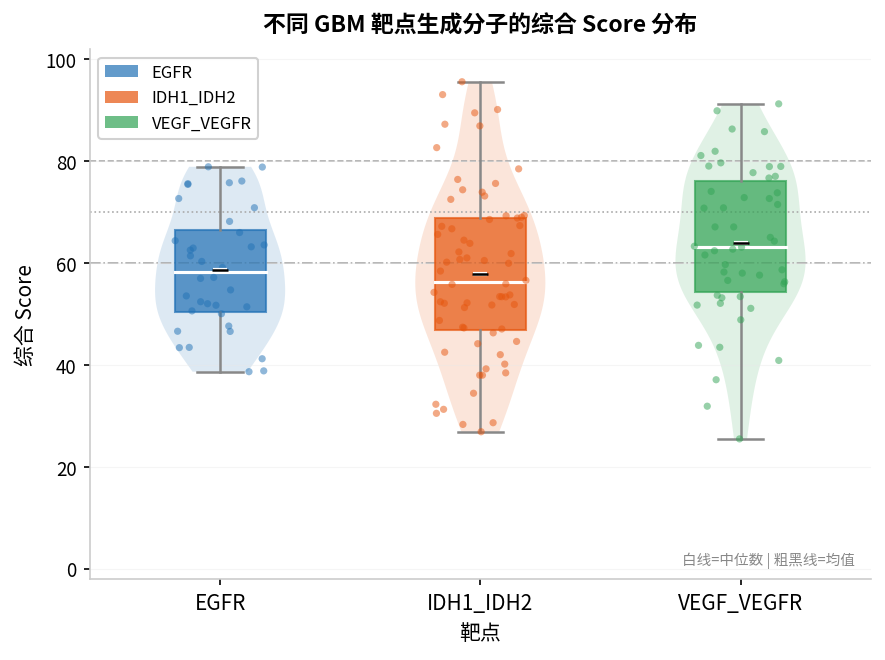
\includegraphics[width=0.8\textwidth]{图片/实验结果可视化图/fig1_score_distribution.zh.png}
    \caption{综合Score分布直方图}\label{fig:score-dist}
\end{figure}

\textbf{结果分析}：VEGF/VEGFR的综合Score分布较为均衡，均值和中位数均高于其他两组，提示该靶点在本计算评价体系下候选分子质量分布更为集中；EGFR和IDH1的分布宽度较窄，整体评分偏低，提示这两个靶点在本框架下的生成分子多集中于中低分层级。

这一分布差异的可能原因包括：（1）VEGF/VEGFR靶点的生成分子在理化性质上更接近CNS药物的典型特征~\cite{Ertl2000,Pardridge2012}；（2）EGFR靶点的成熟度高~\cite{Fu2025}，但同时也需要更复杂的约束设计~\cite{Fu2025}，在当前框架下生成高质量EGFR配体的难度较大；（3）IDH1靶点的结构约束特殊~\cite{Fu2025}，可能需要更精细的骨架设计。

\subsection{DrugCLIP Score分布}\label{sec:drugclip-dist}

图\ref{fig:drugclip-dist}展示了三个靶点生成分子的DrugCLIP Score分布直方图。

\begin{figure}[htbp]
    \centering
    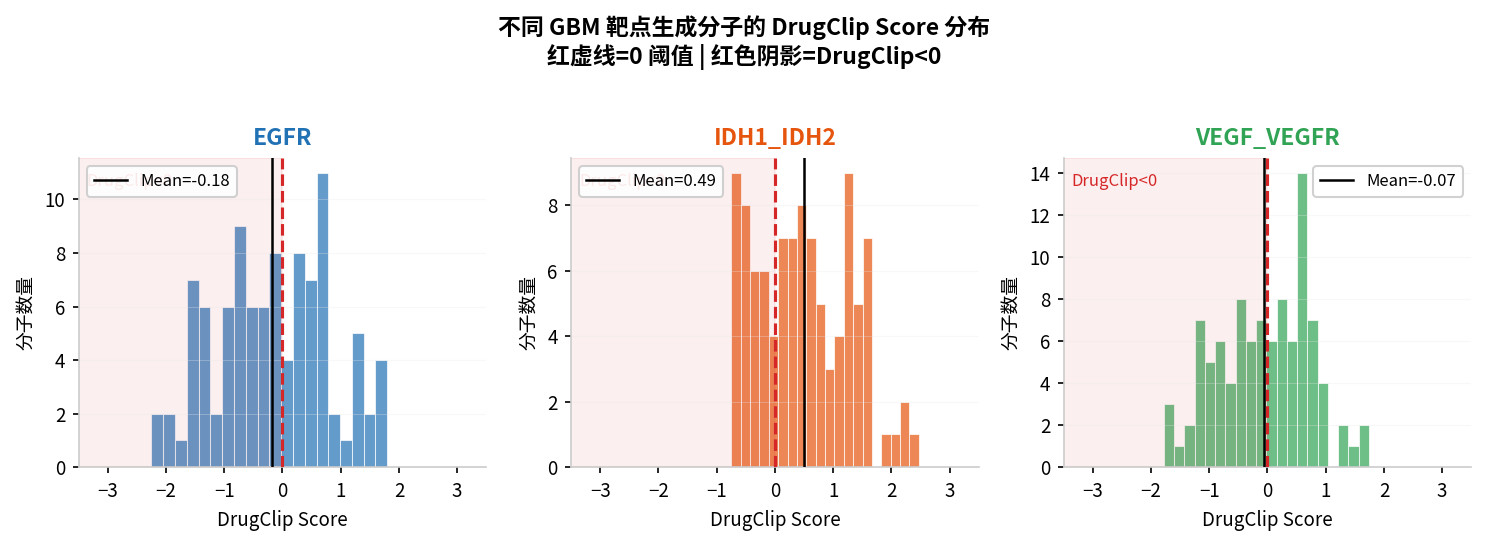
\includegraphics[width=0.8\textwidth]{图片/实验结果可视化图/fig2_drugclip_distribution.zh.png}
    \caption{DrugCLIP Score分布直方图}\label{fig:drugclip-dist}
\end{figure}

\begin{table}[htbp]
    \centering
    \caption{DrugCLIP Score统计数据}\label{tab:drugclip-stats}
    \begin{tabular}{lcccc}
        \toprule
        \textbf{靶点} & \textbf{DrugCLIP>0分子数} & \textbf{均值} & \textbf{标准差} & \textbf{最高值} \\
        \midrule
        EGFR & 43 & 0.57 & 0.37 & 1.61 \\
        IDH1 & 67 & \textbf{0.93} & 0.60 & \textbf{2.47} \\
        VEGF & 48 & 0.62 & 0.38 & 1.74 \\
        \textbf{三靶点合计} & \textbf{158} & \textbf{0.74} & - & - \\
        \bottomrule
    \end{tabular}
\end{table}

\textbf{结果分析}：IDH1靶点的DrugCLIP均值最高（0.93），是三个靶点中预测活性最为突出的~\cite{Gao2023}。这一现象可能与以下因素有关：（1）IDH1靶点的训练数据相对丰富~\cite{Gao2023}；（2）IDH1突变位点（R132H）的口袋结构相对规则~\cite{Fu2025}，适合DrugCLIP模型的语义匹配~\cite{Gao2023}；（3）IDH1生成分子的理化性质更接近训练数据分布~\cite{Gao2023}。

从医学背景来看~\cite{Fu2025}，IDH1/IDH2是GBM分子分型的重要标志物，约10\%的GBM携带IDH突变~\cite{Fu2025}。IDH1突变体通过产生2-羟基戊二酸（2-HG）影响肿瘤代谢~\cite{Fu2025}。由于IDH1在GBM中的重要性已有较多研究~\cite{Fu2025}，相关抑制剂结构信息较为丰富~\cite{Fu2025}，这可能使得模型能够学习到较为有效的分子模式。

\textbf{靶点差异分析}：EGFR的DrugCLIP均值（0.57）相对较低，可能原因包括：（1）EGFR是GBM中研究最成熟的靶点~\cite{Fu2025}，已有大量结构和抑制剂数据~\cite{Fu2025}，模型可能倾向于生成与已知化合物相似的结构，导致与训练数据的差异较大~\cite{Gao2023}；（2）EGFR靶向治疗在GBM中面临 BBB 穿透受限、EGFRvIII 等异常形式以及旁路信号激活等多重挑战~\cite{Fu2025}，在满足这些复杂约束的同时保持高预测活性具有较大难度~\cite{Fu2025}。

\subsection{Vina对接分数分布}\label{sec:vina-dist}

图\ref{fig:vina-dist}展示了DrugCLIP>0分子的Vina对接分数分布箱线图。

\begin{figure}[htbp]
    \centering
    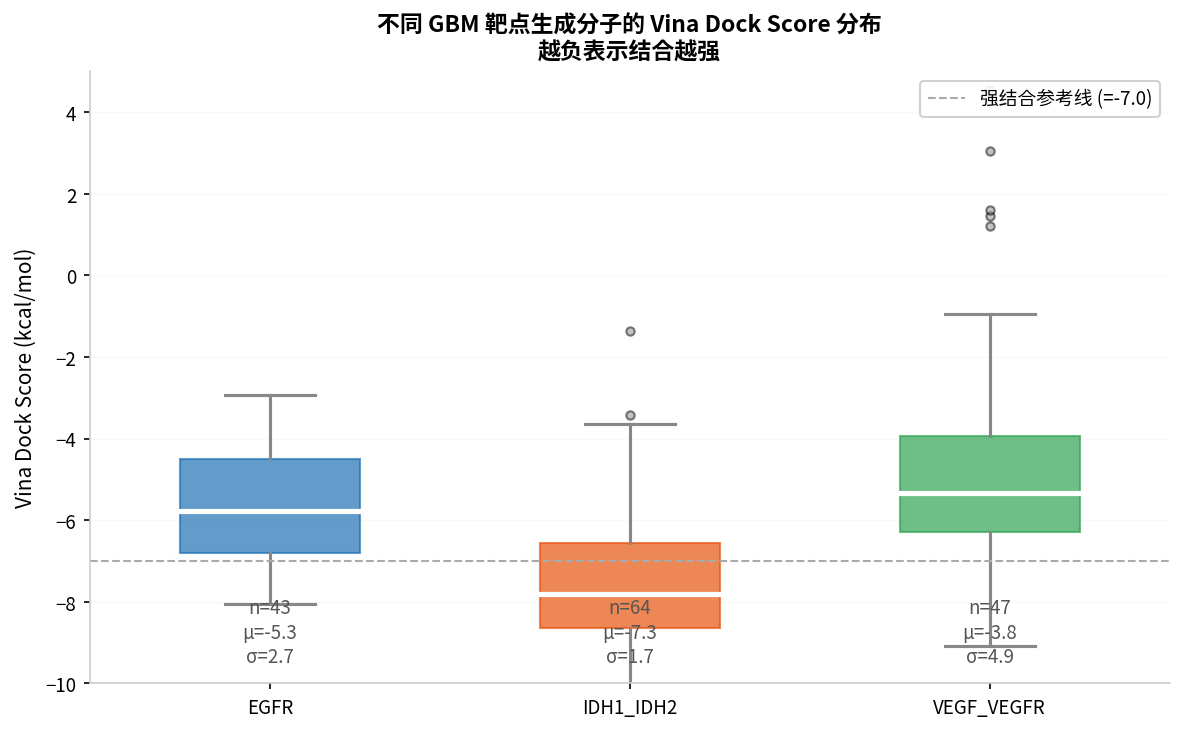
\includegraphics[width=0.8\textwidth]{图片/实验结果可视化图/fig3_vina_distribution.zh.png}
    \caption{Vina对接分数分布箱线图}\label{fig:vina-dist}
\end{figure}

\begin{table}[htbp]
    \centering
    \caption{Vina对接分数统计数据}\label{tab:vina-stats}
    \begin{tabular}{lccc}
        \toprule
        \textbf{靶点} & \textbf{Vina均值(kcal/mol)} & \textbf{标准差} & \textbf{与强结合参考阈值比较} \\
        \midrule
        EGFR & -5.78 & 2.67 & 未达到（< -7.0） \\
        IDH1 & \textbf{-7.82} & 1.73 & \textbf{已达到}（< -7.0） \\
        VEGF & -5.34 & 4.88 & 未达到（< -7.0） \\
        \bottomrule
    \end{tabular}
\end{table}

\textbf{结果分析}：IDH1的Vina均值（-7.82 kcal/mol）达到预设强结合参考阈值（-7.0 kcal/mol）~\cite{Trott2010}，是三个靶点中唯一达到该阈值的。这提示在当前对接参数和打分函数下~\cite{Trott2010}，IDH1靶点的生成分子与靶点蛋白的预测结合构象相对稳定~\cite{Trott2010}。VEGF的Vina标准差最大（4.88），存在明显的正向离群点，可能与部分生成分子的对接构象不稳定有关~\cite{Trott2010}。

从医学背景分析~\cite{Fu2025}：（1）IDH1突变体（R132H）的活性位点结构相对明确~\cite{Fu2025}，口袋形状和大小适合小分子抑制剂结合~\cite{Fu2025}，这可能是IDH1 Vina分数较优的结构基础；（2）VEGF/VEGFR靶点的结合口袋较大且柔性较强~\cite{Fu2025}，对接结果的不确定性较高~\cite{Trott2010}，这可能解释VEGF Vina分数的较大波动~\cite{Trott2010}；（3）EGFR的ATP结合位点已被广泛研究~\cite{Fu2025}，但 GBM 中常见的 EGFR 扩增和 EGFRvIII 等异常形式~\cite{Fu2025}增加了分子设计的复杂性~\cite{Fu2025}。

\textbf{需要说明的是}：Vina分数是经验打分~\cite{Trott2010}，不代表实验结合自由能，对接分数较优仅表示预测的结合构象在当前打分函数下相对稳定~\cite{Trott2010}。

需要说明的是，箱线图中的Vina对接分数均值反映的是全部生成分子的整体分布，而非最终高分候选分子的质量。由于本文在综合评分中赋予Vina对接分数较高权重，高分候选分子通常需要具备较优的对接表现，其Vina分数一般能够达到或接近强结合参考阈值。因此，整体均值偏高并不必然意味着筛选出的高分候选分子结合能力不足，而应结合分层结果和Top候选分子的具体对接分数综合判断。

\subsection{DrugCLIP与Vina相关性分析}\label{sec:drugclip-vina-corr}

图\ref{fig:drugclip-vs-vina}展示了DrugCLIP Score与Vina对接分数的散点图。

\begin{figure}[htbp]
    \centering
    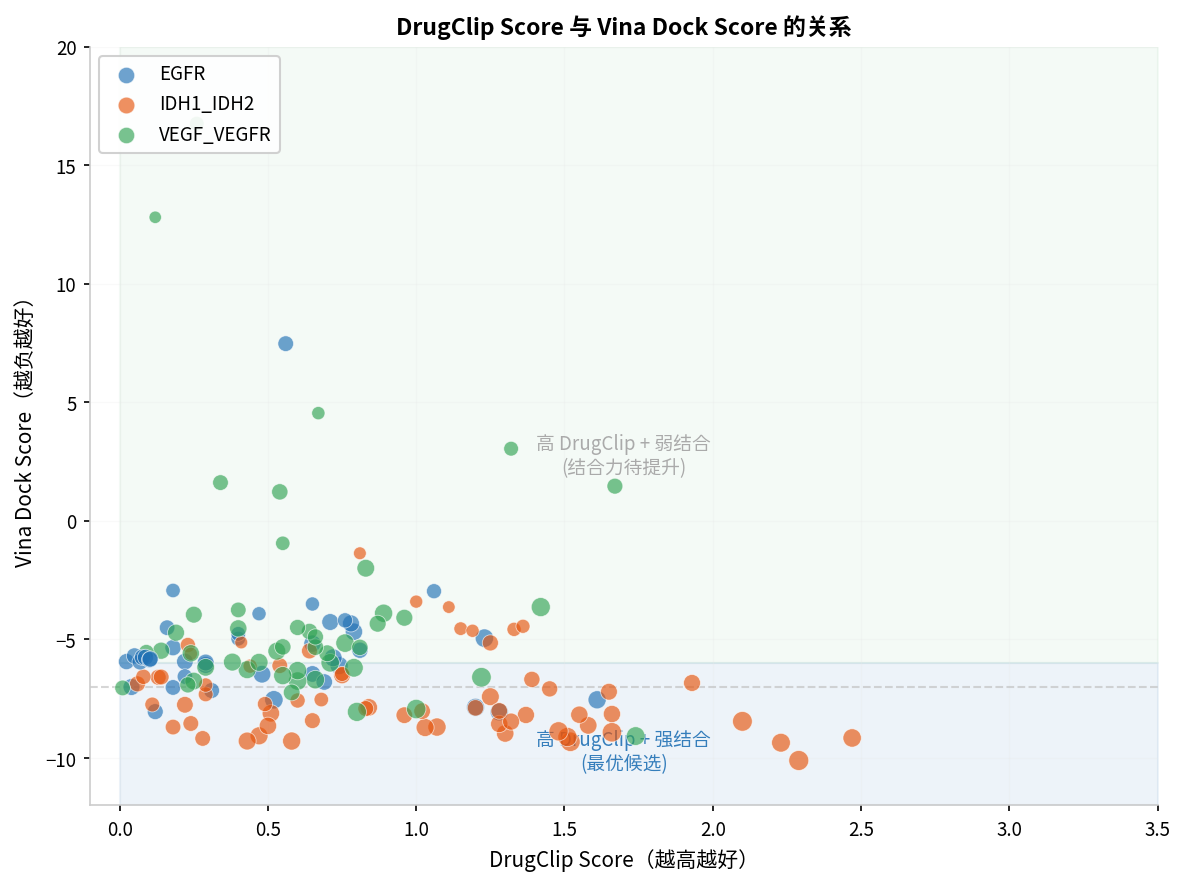
\includegraphics[width=0.8\textwidth]{图片/实验结果可视化图/fig4_drugclip_vs_vina.zh.png}
    \caption{DrugCLIP与Vina散点图}\label{fig:drugclip-vs-vina}
\end{figure}

\textbf{结果分析}：DrugCLIP与Vina之间存在弱负相关（DrugCLIP越高，Vina越负），说明语义预测活性和物理对接打分具有一定一致性~\cite{Gao2023}，但两者并不完全等价~\cite{Gao2023}。这一现象的可能原因包括：（1）DrugCLIP基于语义相似度~\cite{Gao2023}，而Vina基于三维构象打分~\cite{Trott2010}；（2）两者在不同的数据分布上训练~\cite{Gao2023,Trott2010}；（3）Vina打分受蛋白口袋适应性影响~\cite{Trott2010}。因此，多指标联合评估是必要的~\cite{Gao2023,Trott2010}。

这一相关性分析验证了本文同时使用DrugCLIP和Vina两个独立评估维度的合理性~\cite{Gao2023,Trott2010}。

\subsection{BBB穿透性预测结果}\label{sec:bbb-pass}

图\ref{fig:bbb-pass}展示了三个靶点的BBB穿透性预测通过率。

\begin{figure}[htbp]
    \centering
    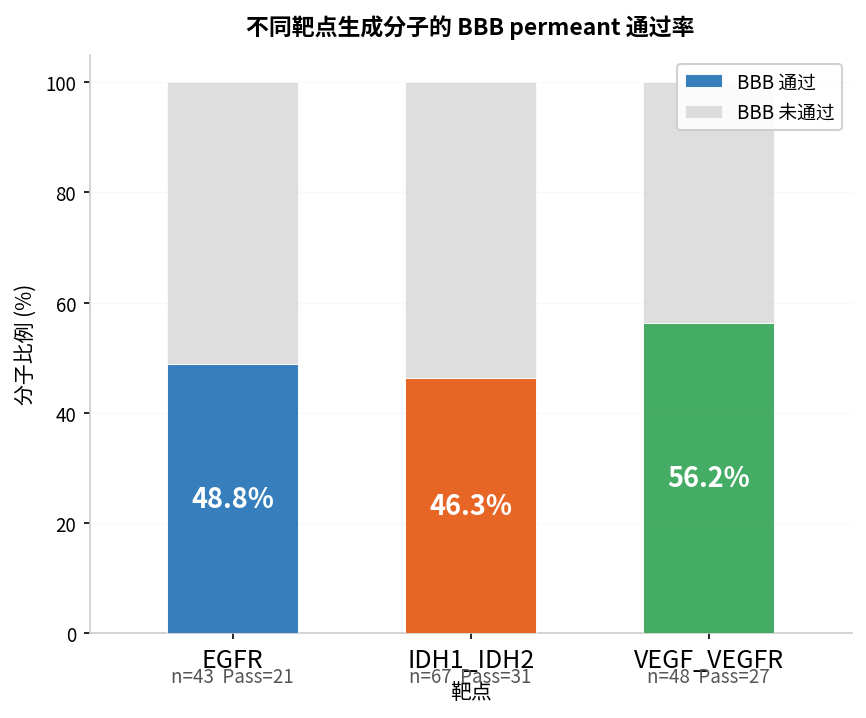
\includegraphics[width=0.8\textwidth]{图片/实验结果可视化图/fig5_bbb_pass_rate.zh.png}
    \caption{BBB穿透性预测通过率堆叠条形图}\label{fig:bbb-pass}
\end{figure}

\begin{table}[htbp]
    \centering
    \caption{BBB穿透性预测统计数据}\label{tab:bbb-stats}
    \begin{tabular}{lccc}
        \toprule
        \textbf{靶点} & \textbf{DrugCLIP>0分子数} & \textbf{BBB预测通过数} & \textbf{BBB预测通过率} \\
        \midrule
        EGFR & 43 & 21 & 48.8\% \\
        IDH1\_IDH2 & 67 & 31 & 46.3\% \\
        VEGF\_VEGFR & 48 & 27 & 56.2\% \\
        \textbf{三靶点合计} & \textbf{158} & \textbf{79} & \textbf{50.0\%} \\
        \bottomrule
    \end{tabular}
\end{table}

\textbf{结果分析}：三个靶点的BBB穿透性预测通过率均未超过60\%，说明BBB穿透仍是GBM分子设计面临的主要难点之一~\cite{Pardridge2012}。VEGF/VEGFR的预测通过率相对最高（56.2\%），可能与该靶点生成分子的MW偏小、TPSA偏小有关~\cite{Ertl2000}。

从CNS药物设计的角度分析~\cite{Pardridge2012}：（1）BBB穿透需要满足严格的理化约束~\cite{Pardridge2012}，MW<450 Da、TPSA<90 \AA$^2$、LogP 1-4~\cite{Ertl2000,Pardridge2012}，这些约束限制了生成分子的化学空间；（2）VEGF/VEGFR靶点主要与血管生成相关~\cite{Fu2025}，相关抑制剂多为小分子化合物~\cite{Fu2025}，这可能使得生成分子更符合BBB理化要求；（3）EGFR和IDH1靶点的抑制剂结构相对较大~\cite{Fu2025}，满足BBB约束的同时保持靶点活性具有挑战性。

\section{消融实验分析}\label{sec:ablation}

消融实验用于量化各核心模块对生成质量的贡献。本文设计了7组消融实验，如表\ref{tab:ablation-config}所示。

\textbf{实验目的}：通过逐个移除关键模块，量化每个模块对最终生成质量的贡献，验证各模块的必要性。

\textbf{实验设计原因}：（1）CoT-ToT推理用于结构化生成~\cite{Wei2022,Yao2023}，移除后应导致生成质量下降；（2）物理评估用于剪枝不合格分子~\cite{Trott2010}，移除后应导致不合格分子进入结果集；（3）反馈机制用于动态调整生成方向~\cite{Yao2023}，移除后应导致重复生成低质量分子；（4）GBM知识库和LoRA用于领域适配~\cite{hu2022lora}，移除后应导致生成分子偏离GBM特异化学空间。

\begin{table}[htbp]
    \centering
    \caption{消融实验配置}\label{tab:ablation-config}
    \begin{tabular}{lll}
        \toprule
        \textbf{实验编号} & \textbf{实验名称} & \textbf{消融内容} \\
        \midrule
        Ablation-1 & 无CoT和ToT推理 & 移除CoT推理模板和ToT搜索，仅直接生成完整分子 \\
        Ablation-2 & 无ToT推理（仅CoT） & 移除ToT多分支搜索，保留CoT结构化推理 \\
        Ablation-3 & 无物理反馈 & 移除物理引擎反馈 \\
        Ablation-4 & 无物理评估 & 移除整个物理评估环节 \\
        Ablation-5 & 无领域知识 & 移除GBM知识库注入 \\
        Ablation-6 & 无GBM LoRA & 仅使用通用底层生成模型适配器 \\
        Ablation-7 & 基线模型 & 不使用任何适配器 \\
        \bottomrule
    \end{tabular}
\end{table}

图\ref{fig:ablation-score}和图\ref{fig:ablation-relative}展示了消融实验结果。

\begin{figure}[htbp]
    \centering
    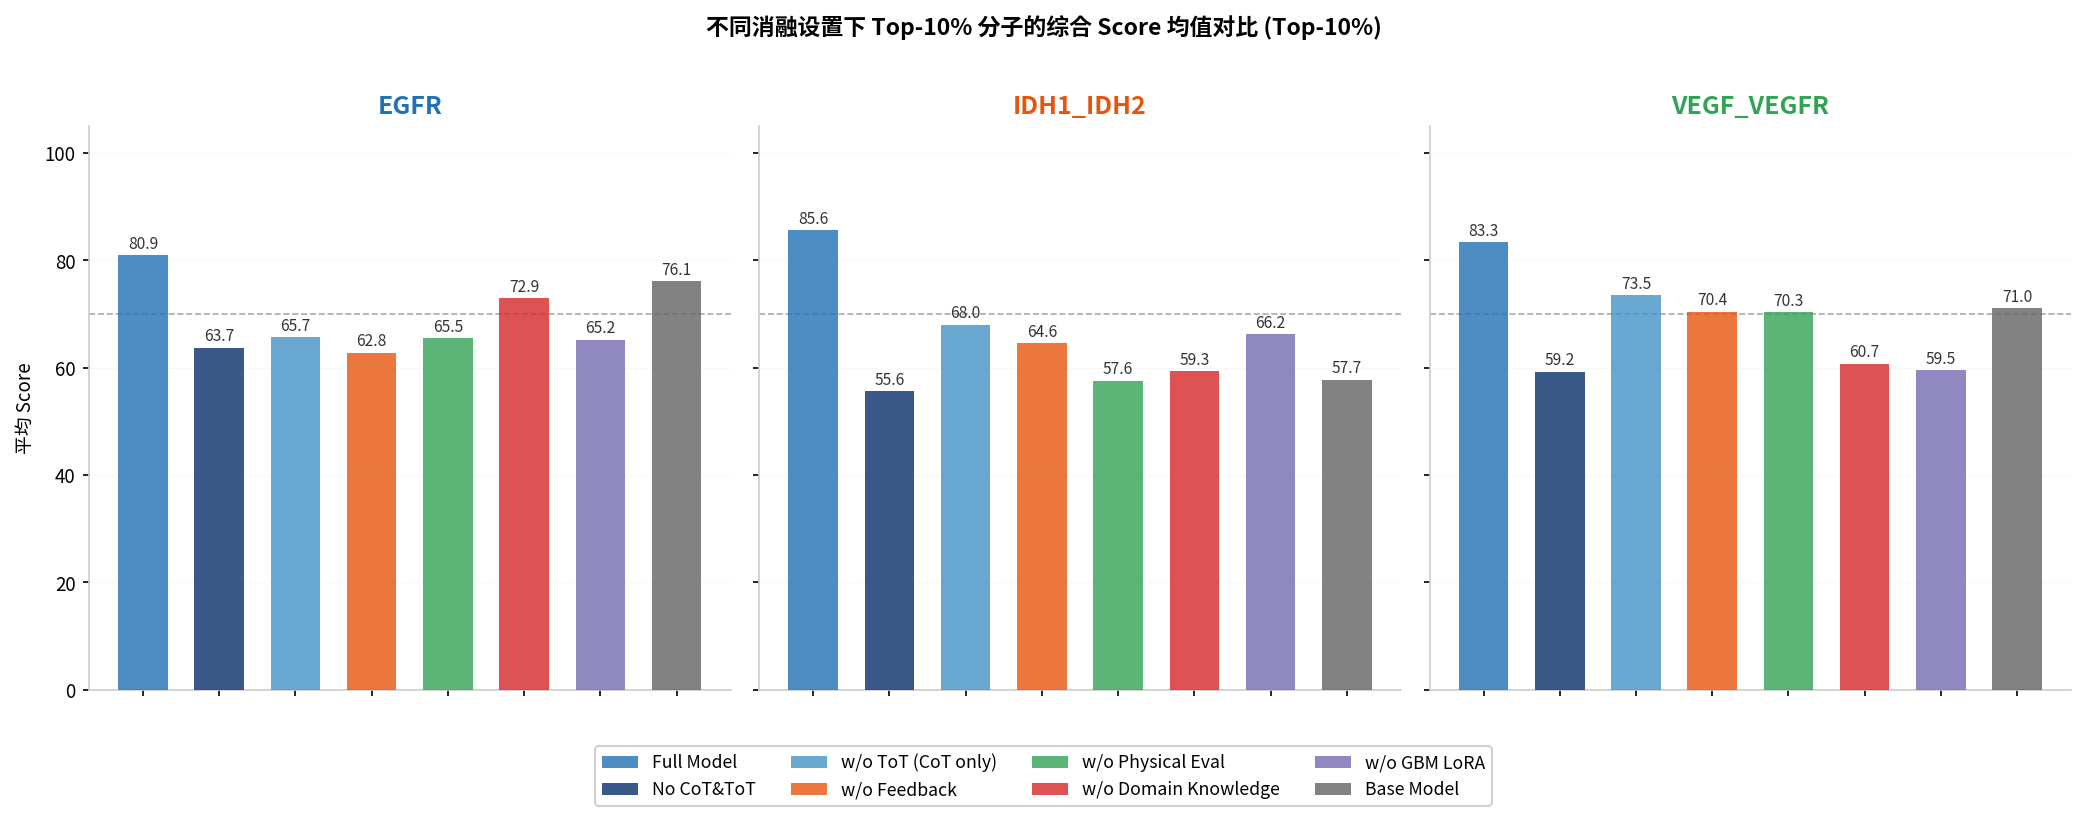
\includegraphics[width=0.8\textwidth]{图片/实验结果可视化图/fig8_ablation_score_comparison.zh.png}
    \caption{消融实验DrugCLIP均值对比}\label{fig:ablation-score}
\end{figure}

\begin{figure}[htbp]
    \centering
    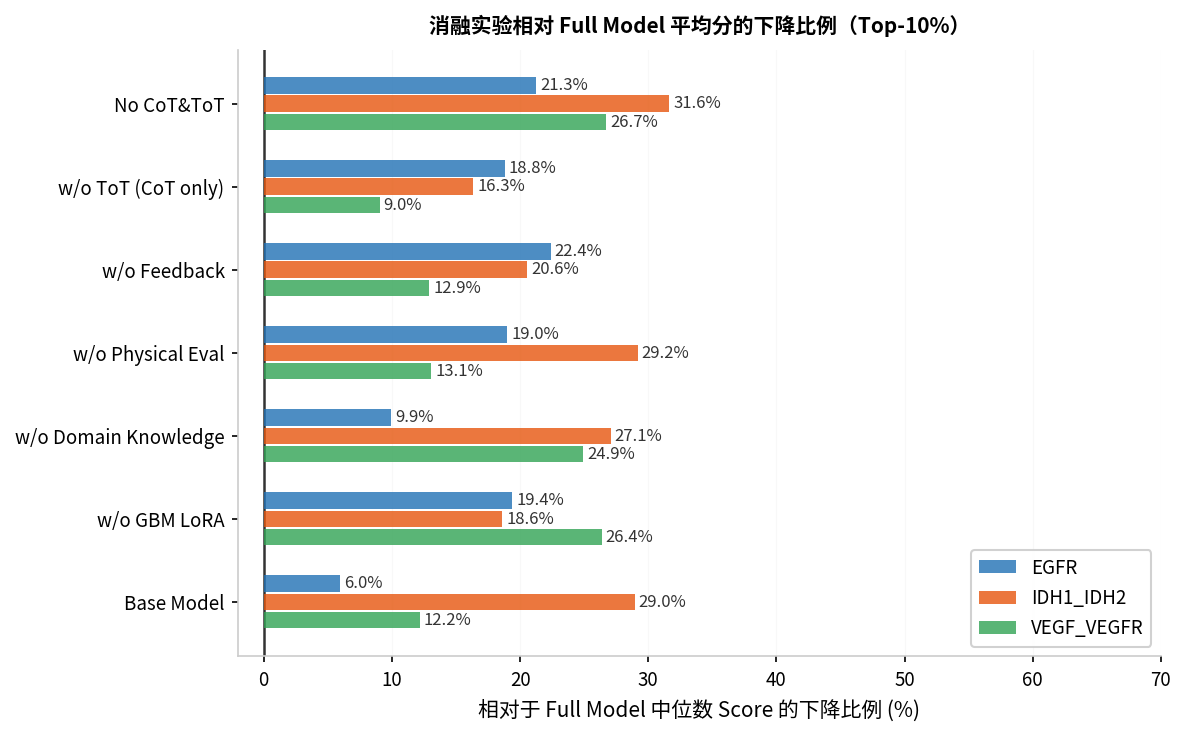
\includegraphics[width=0.8\textwidth]{图片/实验结果可视化图/fig9_ablation_relative_drop.zh.png}
    \caption{Top分子质量相对下降幅度}\label{fig:ablation-relative}
\end{figure}

\begin{table}[htbp]
    \centering
    \caption{消融实验DrugCLIP均值下降统计}\label{tab:ablation-drop}
    \begin{tabular}{lcc}
        \toprule
        \textbf{消融设置} & \textbf{DrugCLIP均值下降} & \textbf{说明} \\
        \midrule
        无CoT和ToT推理 & \textbf{26.5\%} & 最大降幅 \\
        无ToT推理（仅CoT） & \textbf{15.3\%} & 第二大降幅（CoT单独贡献约11.2\%） \\
        无物理评估 & \textbf{24.0\%} & 第三大降幅 \\
        无反馈 & \textbf{20.1\%} & 第四大降幅 \\
        无GBM LoRA & 10.8\% & - \\
        无领域知识 & 9.5\% & - \\
        基线模型 & \textbf{45.9\%} & 远超其他消融 \\
        \bottomrule
    \end{tabular}
\end{table}

图\ref{fig:drugclip-ratio}展示了DrugCLIP>0分子占比的对比结果。

\begin{figure}[htbp]
    \centering
    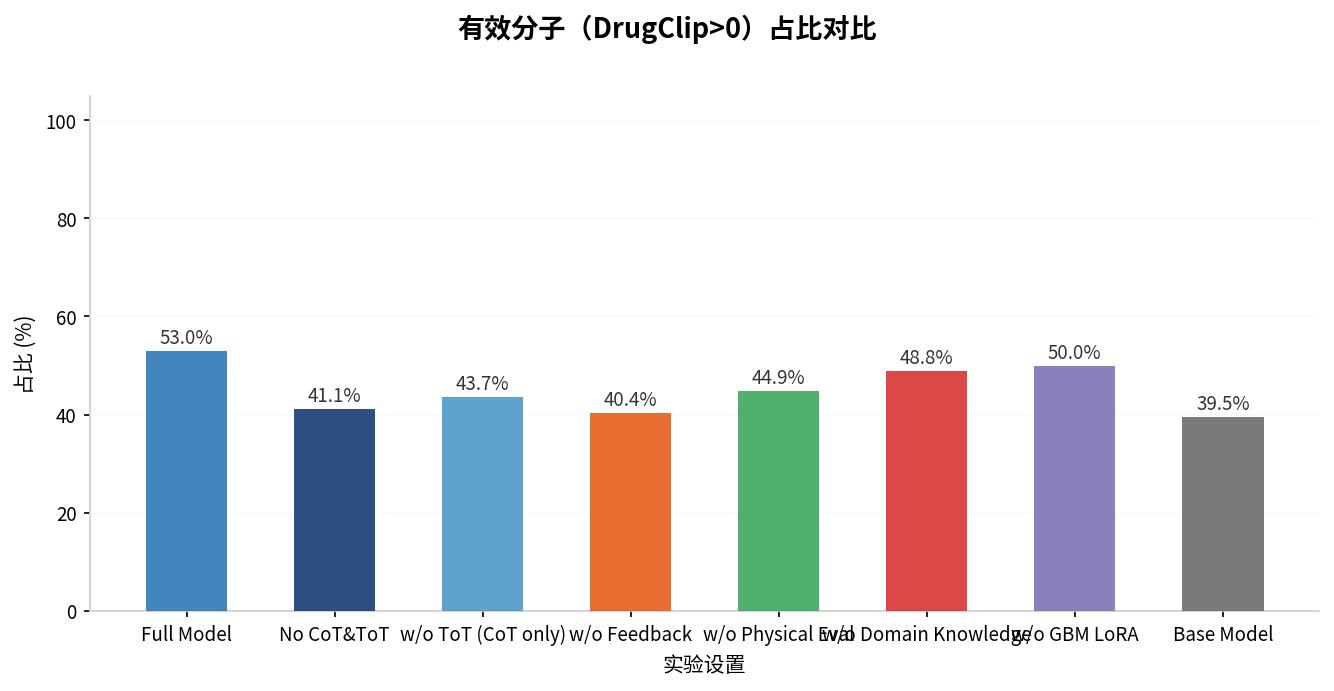
\includegraphics[width=0.8\textwidth]{图片/实验结果可视化图/fig12_drugclip_ratio.zh.png}
    \caption{DrugCLIP>0分子占比对比}\label{fig:drugclip-ratio}
\end{figure}

%\begin{table}[htbp]
%    \centering
%    \caption{DrugCLIP>0分子占比对比}\label{tab:drugclip-ratio}
%    \begin{tabular}{lc}
%        \toprule
%        \textbf{方法} & \textbf{DrugCLIP>0分子占比} \\
%        \midrule
%        GBM-PharmaMind（本文框架） & \textbf{53.0\%} \\
%        LlaSMol-Mistral-7B & 39\% \\
%        Top-K & 38\% \\
%        \bottomrule
%    \end{tabular}
%\end{table}

\textbf{结果分析}：

\textbf{（1）无CoT和ToT推理下降最大（26.5\%）}：这一结果符合预期~\cite{Wei2022,Yao2023}。CoT推理通过结构化步骤引导模型逐步推理~\cite{Wei2022}，将"生成什么分子"这一模糊目标分解为可操作的具体子任务~\cite{Wei2022}；ToT搜索通过多分支探索~\cite{Yao2023}，避免了单一路径生成陷入局部最优~\cite{Yao2023}。两者的协同作用使得生成质量和多样性均有提升~\cite{Yao2023}。

\textbf{设计原因}：分子设计是一个多约束、多阶段的复杂任务~\cite{Zhou2019Exp}。如果没有CoT-ToT~\cite{Wei2022,Yao2023}，模型可能一次性输出难以检验的完整分子~\cite{Wei2022}，难以追溯设计依据~\cite{Wei2022}，也可能忽略其他可能的分子设计方向~\cite{Yao2023}。

\textbf{（2）无物理评估下降显著（24.0\%）}：物理评估模块（Vina对接、DILI/hERG警报、BBB预测）是过滤不合格分子的核心机制~\cite{Trott2010,Aronov2008}。移除物理评估后，大量理化性质不合格的分子进入最终结果集，导致整体评分下降。

\textbf{设计原因}：如果没有物理评估模块~\cite{Trott2010}，LLM生成的分子可能存在化学有效性问题~\cite{Bagal2021}或理化性质不符合BBB要求~\cite{Pardridge2012}。物理评估提供了量化的反馈信号，使得系统能够识别并过滤不合格分子~\cite{Trott2010}。

\textbf{（3）无反馈下降第三（20.1\%）}：物理评估反馈使得生成过程能够根据评估结果动态调整~\cite{Yao2023}。没有反馈时，模型无法从上一轮的失败中学习~\cite{Yao2023}，导致同一类型的低质量分子被反复生成~\cite{Yao2023}。

\textbf{设计原因}：闭环反馈是实现"生成-评估-优化"迭代优化的关键~\cite{Yao2023}。如果没有反馈机制~\cite{Yao2023}，每一轮生成都是独立的~\cite{Yao2023}，无法利用上一轮的评估结果来指导下一轮的生成方向~\cite{Yao2023}。

\textbf{（4）无GBM LoRA和无领域知识下降较小但仍显著}：GBM LoRA适配和领域知识注入分别带来10.8\%和9.5\%的提升~\cite{hu2022lora}。虽然不如CoT-ToT和物理评估的贡献大~\cite{hu2022lora}，但两者合计接近20\%，说明领域适配对最终质量有不可忽视的贡献~\cite{hu2022lora}。

\textbf{靶点差异分析}：对于EGFR这类成熟靶点~\cite{Fu2025}，通用模型可能已经学到较多相关结构模式~\cite{Fu2025}，因此领域知识增益可能较小；对于IDH1/IDH2或VEGF/VEGFR~\cite{Fu2025}，领域知识可能提供更关键的疾病约束和靶点特异性提示~\cite{Fu2025}。

\textbf{（5）基线模型下降最大（45.9\%）}：基线模型（无任何适配器）同时去除了领域知识注入、GBM LoRA和CoT-ToT~\cite{hu2022lora}，导致性能大幅退化~\cite{hu2022lora}。

\section{对比实验分析}\label{sec:comparison}

为验证本文方法的有效性，本文与以下分子生成方法在相同靶点（EGFR、VEGF/VEGFR、IDH1/IDH2）上进行了对比实验。所有方法采用相同的分子预处理流程（去重、SMILES 有效性过滤）以及相同的评估指标，以确保对比的公平性。

\begin{table}[htbp]
    \centering
    \caption{对比方法说明}\label{tab:comparison-methods}
    \begin{tabular}{lp{12cm}}
        \toprule
        \textbf{方法} & \textbf{模型定位与技术特点} \\
        \midrule
        GBM-PharmaMind（本文） & 以 Qwen2-7B-Instruct 为基座模型，结合 Llamole 分子图—文本协同生成、GBM 领域知识库注入、GBM LoRA 适配与 CoT-ToT 协同推理，并引入 DrugCLIP、AutoDock Vina、BBB 经验模型、DILI/hERG 结构警报和 MPO Reward 的物理反馈闭环 \\
        LlaSMol-Mistral-7B~\cite{Yu2024} & 基于 Mistral-7B 微调的化学领域指令模型~\cite{Yu2024}，擅长化学问答与性质预测指令，不具备疾病靶点约束注入机制，分子生成依赖通用指令而非结构化领域知识 \\
        PlayMolecule AI~\cite{rusinko2024aiddison} & 商业化分子设计平台~\cite{rusinko2024aiddison}，基于已知药物母核进行局部结构微调~\cite{torrensfontanals2024playmolecule}，对给定靶点生成分子时倾向于骨架收敛至参考配体样结构，分子量普遍偏大（$\sim$500--530 Da） \\
        Llamole Qwen-7b~\cite{liu2025multimodal} & 原始 Llamole 模型~\cite{liu2025multimodal}，针对逆合成路径规划任务训练~\cite{liu2025multimodal}，无 GBM 领域知识注入、无 LoRA 适配，无物理反馈闭环 \\
        LLaMA-MolInst-Molecule-7B & 基于 Decapoda-LLaMA-7B 加载 MolInst LoRA 适配器的分子指令模型，SMILES 输出格式使用 atom-bond notation，成功率极低（EGFR 6/50，IDH1 2/50，VEGF 3/50），生成分子大量含非法化学符号，无法参与指标对比 \\
        \bottomrule
    \end{tabular}
\end{table}

\begin{table}[htbp]
    \centering
    \caption{各方法综合评分 Top-10 指标对比}\label{tab:comparison-top10}
    \begin{threeparttable}
    \begin{tabular}{lcccccc}
        \toprule
        \textbf{方法} & \textbf{靶点} & \textbf{N} &
        \textbf{Top-1} & \textbf{Top-3 均分} & \textbf{Top-10 均分} \\
        \midrule
        \multirow{3}*{GBM-PharmaMind（本文）} & EGFR & 43 & 78.92 & 77.97 & 73.86 \\
        & IDH1 & 67 & 95.61 & 92.95 & 81.63 \\
        & VEGF & 48 & 91.27 & 89.17 & 79.19 \\
        \cmidrule(lr){1-6}
        \multirow{3}*{LlaSMol~\cite{Yu2024}} & EGFR & 15 & 70.41 & 69.30 & 59.69 \\
        & IDH1 & 21 & 96.04 & 90.17 & 67.69 \\
        & VEGF & 23 & 91.57 & 88.34 & 76.30 \\
        \cmidrule(lr){1-6}
        \multirow{3}*{PlayMolecule AI~\cite{rusinko2024aiddison}} & EGFR & 50 & 77.54 & 76.96 & 74.57 \\
        & IDH1 & 41 & 77.73 & 76.72 & 69.93 \\
        & VEGF & 50 & 81.71 & 80.90 & 78.31 \\
        \cmidrule(lr){1-6}
        \multirow{3}*{Llamole~\cite{liu2025multimodal}} & EGFR & 3 & 80.00 & 54.23 & --\tnote{*} \\
        & IDH1 & 15 & 83.57 & 81.70 & 60.16 \\
        & VEGF & 3 & 74.51 & 64.85 & --\tnote{*} \\
        \bottomrule
    \end{tabular}
    \begin{tablenotes}
        \item[*] 有效分子数不足 10 个，Top-10 均分不具统计意义，以 -- 标记。
    \end{tablenotes}
    \end{threeparttable}
\end{table}

\begin{itemize}
    \setlength{\itemsep}{0.2em}
    \item \textbf{GBM-PharmaMind 在 EGFR 靶点的 Top-1、Top-3 和 Top-10 综合分上表现较好；在 IDH1 靶点上，虽然 Top-1 略低于 LlaSMol，但 Top-10 均分具有明显优势。}如表~\ref{tab:comparison-top10} 所示，在 EGFR 靶点上 GBM-PharmaMind 的 Top-1 综合分（78.92）领先 LlaSMol（70.41）约 8.5 分，Top-3 均分（77.97）领先约 8.7 分，Top-10 均分（73.86）领先约 14.2 分，说明本文方法的优势主要体现在 EGFR 靶点的中高分候选分子质量上。在 IDH1 靶点上，GBM-PharmaMind 的 Top-1 综合分（95.61）略低于 LlaSMol（96.04），差异 $< 0.5$ 分；但 Top-10 均分（81.63）明显高于 LlaSMol（67.69），说明本文方法在 IDH1 靶点上的优势主要体现在中高分候选分子的整体质量，而非单个最高分分子。在 VEGF 靶点上两者 Top-1 综合分几乎持平（差异 $< 0.5$ 分），Top-3 和 Top-10 均分也相近，说明 VEGF 并非本文方法全面领先的靶点。综合而言，GBM-PharmaMind 在部分靶点的高分候选分子生成方面表现出一定优势，但该优势并非体现在所有指标或所有靶点上。因此，对比实验结果应理解为本文方法在特定靶点和特定评分口径下的有效性验证，而非全面优于所有对比方法。

    \item \textbf{LlaSMol 在三个靶点上共生成 59 个有效分子，DrugCLIP $> 0$ 分子占比为 100\%，说明其生成分子的理化性质稳定，均在 DrugCLIP 的正预测区间内。}然而，LlaSMol 仅生成 15--23 个有效分子，远少于 GBM-PharmaMind 的 43--67 个，且 Top-10 均分在三个靶点上均低于 GBM-PharmaMind。这说明 LlaSMol 擅长生成理化性质合格的分子，但在靶点语义匹配活性的整体水平上弱于 GBM-PharmaMind。从本质分析，LlaSMol 的训练任务以化学指令为主~\cite{Yu2024}，缺乏疾病靶点知识注入和结构化推理机制，导致其在根据靶点信息生成候选分子的任务中条件生成能力受限。

    \item \textbf{PlayMolecule AI 在各靶点上 Top-10 均分表现均衡但缺乏多样性。}PlayMolecule AI 生成分子的 DrugCLIP $> 0$ 占比达 100\%（141/141），Top-10 均分在三个靶点上均高于 LlaSMol 和 Llamole，与 GBM-PharmaMind 接近（EGFR 74.57 vs 73.86，IDH1 69.93 vs 81.63，VEGF 78.31 vs 79.19）。然而，其 Top-1 综合分均低于 GBM-PharmaMind 和 LlaSMol，说明其生成分子质量较为均衡但缺乏顶尖分子。PlayMolecule AI 生成结果为已知药物母核的局部修饰变体，分子骨架收敛至参考配体样结构，缺乏创新性分子骨架的多样性，因此不适合作为根据靶点信息生成创新候选分子场景下的生成模型对比基准。

    \item \textbf{Llamole 有效分子数严重不足，结论不具统计意义。}原始 Llamole 在 EGFR 和 VEGF 上仅分别生成 3 个 DrugCLIP $> 0$ 分子，IDH1 上生成 15 个，其 Top-1 综合分虽高（EGFR 80.00，IDH1 83.57，VEGF 74.51），但 Top-10 均分在 EGFR 和 VEGF 上因 N $< 10$ 而不可比，IDH1 的 Top-10 均分（60.16）也大幅低于 GBM-PharmaMind（81.63）。这直接验证了 GBM-PharmaMind 中 GBM LoRA 适配、领域知识注入和物理反馈闭环的必要性。原始 Llamole 针对逆合成规划训练~\cite{liu2025multimodal}，缺乏靶点条件约束注入，因此大多数生成分子无法通过 DrugCLIP 筛选阈值。

    \item \textbf{LLaMA-MolInst-Molecule-7B 无法参与指标对比。}该模型生成成功率极低（EGFR 6/50，IDH1 2/50，VEGF 3/50），且大量输出包含非标准化学符号（如 \texttt{NNNCCCCON}、\texttt{-O-[Al+1][Al-1]} 等），无法通过 RDKit 的 SMILES 标准化验证，因此未纳入表~\ref{tab:comparison-top10} 的指标对比。从本质分析，Decapoda-LLaMA-7B 基础能力有限~\cite{Touvron2023LLaMA}，LoRA 适配层参数量较少（相比 Qwen2-7B），且未引入分子图生成机制，导致化学有效输出率极低。

\end{itemize}

\textbf{对比实验小结}：GBM-PharmaMind 在 EGFR 靶点的 Top-1、Top-3 和 Top-10 综合分上表现较好；在 IDH1 靶点上，虽然 Top-1 略低于 LlaSMol，但 Top-10 均分（81.63）明显高于 LlaSMol（67.69），优势约 13.9 分，说明本文方法的优势主要体现在中高分候选分子的整体质量，而非所有靶点的单个最高分分子。PlayMolecule AI 和 LlaSMol 生成规模有限且分子多样性差；原始 Llamole 因缺乏领域适配而有效分子数极少；LLaMA-MolInst-Molecule-7B 因成功率过低而不具可比性。综合而言，GBM-PharmaMind 在部分靶点的高分候选分子生成方面表现出一定优势，但该优势并非体现在所有指标或所有靶点上，其结果应理解为本文方法在特定靶点和特定评分口径下的有效性验证。

\section{本章小结}\label{sec:ch4-summary}

本章在EGFR、VEGF/VEGFR和IDH1/IDH2三个代表性GBM靶点上对本文提出的GBM候选分子生成框架进行了系统性实验验证。

\textbf{主实验结果}（DrugCLIP Score > 0的分子）：
\begin{itemize}
    \item \textbf{IDH1表现较为突出}：DrugCLIP均值0.93（最高），Vina均值-7.82 kcal/mol（唯一达到强结合参考阈值）。这一现象可能与IDH1突变体口袋结构相对规则~\cite{Fu2025}、训练数据相对丰富~\cite{Gao2023}等因素有关。
    \item \textbf{三个靶点BBB穿透性预测通过率相近}（46.3\%$\sim$56.2\%，三靶点合计50.0\%），说明BBB穿透仍是GBM分子设计中的主要瓶颈之一~\cite{Pardridge2012}。
    \item \textbf{三靶点综合}：DrugCLIP均值0.74，按 DrugCLIP$>$0 分子数量加权的 Vina 均值约为 -6.51 kcal/mol，BBB穿透预测通过率50.0\%。
\end{itemize}

\textbf{消融实验量化贡献}（DrugCLIP均值下降百分比）：
\begin{itemize}
    \item 无CoT和ToT推理：26.5\%（最大），说明结构化推理和多分支搜索是生成质量的关键驱动因素~\cite{Wei2022,Yao2023}；
    \item 无物理评估：24.0\%，说明评估模块在过滤不合格分子中的核心作用~\cite{Trott2010}；
    \item 无反馈：20.1\%，说明反馈机制能够持续引导生成质量提升~\cite{Yao2023}；
    \item 无GBM LoRA：10.8\%，说明领域适配对最终质量有正向贡献~\cite{hu2022lora}；
    \item 无领域知识：9.5\%，说明GBM知识库的注入有助于提升生成合理性~\cite{jin2025effective}；
    \item 基线模型：45.9\%，说明各模块协同作用的重要性。
\end{itemize}

\textbf{对比实验结论}：本文方法在 EGFR 和 IDH1 靶点的高分候选分子质量方面具有一定优势：EGFR 靶点 Top-1 综合分（78.92）领先 LlaSMol 约 8.5 分，EGFR 和 IDH1 靶点 Top-10 均分（73.86 和 81.63）分别领先 LlaSMol 约 14.2 分和 13.9 分；有效分子总量（158 个）远超 LlaSMol（59 个）和 Llamole（21 个），表明本文方法兼具分子生成规模与中高分候选分子质量。

需要指出的是，本文所有计算指标均为早期虚拟筛选和候选排序参考~\cite{Trott2010,Clark2000,Gao2023}，不能替代体外活性、毒性和BBB渗透实验验证~\cite{Trott2010,Pardridge2012}。实验结果表明本文方法能够为GBM早期虚拟筛选提供候选分子集合和优先级排序依据~\cite{Li2025DrugPilot}，但候选分子的实际生物学和药学活性需要后续的湿实验确认~\cite{Li2025DrugPilot}。

\chapter{总结与展望}\label{chap:conclusion}

\section{研究工作总结}\label{sec:summary-work}

围绕GBM候选药物分子的计算生成与优化问题，本文构建了GBM-PharmaMind候选药物分子生成框架。该框架以多模态大语言模型和分子图—文本生成模型为基础，将GBM领域知识输入、CoT-ToT协同推理和物理评估反馈统一到同一生成流程中。本文工作可从知识层面、框架层面和评估层面加以概括。

\subsection{GBM多模态知识库构建与注入}\label{sec:work-km}

在候选分子生成任务中，模型能否获得足够明确的疾病背景信息，会直接影响生成结果的针对性。本文围绕GBM药物设计场景，整理了与候选分子生成相关的靶点信息、临床治疗经验、参考分子结构以及CNS药物设计规则，使生成过程能够同时参考GBM疾病背景、血脑屏障相关约束和已知结构经验，从而减少完全依赖通用化学空间采样带来的不确定性。

具体来看，本文构建的知识库并不是单独作为背景资料保存，而是参与到Prompt构造和后续生成控制过程中。GBM靶点信息库用于提供EGFR、VEGFR2、IDH1等靶点的基本背景和设计提示；临床治疗数据库用于补充标准治疗方案、耐药机制和已有治疗经验；分子参考数据库用于提供已知药物或候选分子的结构参照；结构知识库则用于记录BBB穿透相关策略、PAINS警告结构以及基础类药性规则。分散的疾病知识和药物化学经验被转化为生成模型可以读取和利用的约束信息，为后续候选分子生成提供了较稳定的输入基础。

\subsection{CoT-ToT协同推理与分子生成模块}\label{sec:work-cot-tot}

本文在分子生成阶段引入CoT-ToT协同推理，主要是为了避免模型一次性输出完整SMILES时缺少中间控制的问题。GBM候选分子生成需要同时考虑靶点背景、BBB穿透倾向、结构有效性和成药性约束，若直接生成最终分子，模型的骨架选择、片段修饰和结构表达会被混合在同一输出中，后续难以判断问题出现在设计思路还是结构落地环节。因此，本文将生成过程拆分为骨架提议、片段组装和SMILES输出三个阶段，使候选分子的形成过程更加清晰。

在这一过程中，CoT用于组织分子设计的推理顺序，使模型先分析靶点和约束条件，再逐步形成候选结构；ToT用于在不同阶段保留多个候选方向，使生成过程不局限于单一路径。骨架提议阶段关注分子的主体结构和潜在药效团方向，片段组装阶段在已有骨架上进行局部修饰，SMILES输出阶段则将前两步得到的结构设想转化为可计算的分子表示。物理评估模块的结果会被写回后续Prompt，使模型能够根据上一轮生成结果调整后续候选方向。通过这种方式，本文将结构化推理、多分支搜索和外部评价反馈连接到同一生成流程中，提高了候选分子生成过程的可控性。

\subsection{基于结构警报检测与Clark公式的成药性快速评估体系}\label{sec:work-physics}

评估层面，本文建立了结合结构警报检测、BBB经验预测、Vina对接、MPO Reward和TotalScore的计算评价体系。生成阶段的评价结果用于剪枝与反馈，最终阶段则通过TotalScore对候选分子进行综合排序。该体系将药物化学规则和外部计算工具转化为可执行的筛选流程，并通过硬剪枝与Delta Scoring机制在安全性约束和化学空间探索之间进行折中。

\section{主要结论}\label{sec:conclusions}

在EGFR、VEGFR2和IDH1等代表性GBM靶点上的实验结果表明，GBM-PharmaMind能够生成具有一定预测活性、BBB穿透倾向和成药性特征的候选分子。Full Model在DrugCLIP、Vina对接分数和BBB相关指标上整体优于消融模型，说明领域知识输入、LoRA适配、CoT-ToT推理和物理评估反馈均对最终生成质量具有显著贡献。

\section{存在的不足}\label{sec:limitations}

本文主要从计算方法角度构建GBM候选分子生成与优化框架，整体流程已经覆盖知识输入、分阶段生成、物理评估反馈和最终候选排序等环节，但仍存在一定改进空间。首先，当前实验主要围绕EGFR、VEGFR2和IDH1等代表性靶点展开，尚未覆盖更多GBM相关分子亚型和耐药机制，因此框架在更复杂靶点组合下的稳定性仍需进一步分析。其次，最终评估中的Vina Score、ADMET性质等指标主要DrugClip和SwissADME等外部工具，对不同预测模型之间的一致性和适用边界讨论仍不充分。最后，ToT搜索宽度和深度目前采用固定设置，尚未根据中间评价结果动态调整，这在一定程度上限制了搜索过程的自适应能力。

\section{未来研究展望}\label{sec:future}

围绕本文工作，后续研究可以继续从框架扩展、评价体系和搜索策略三个方向推进。在框架扩展方面，可将更多GBM相关通路、分子亚型和突变背景纳入实验，并扩大候选分子生成规模，以检验GBM-PharmaMind在不同任务条件下的稳定性。在评价体系方面，可进一步引入更精细的BBB预测模型、P-gp风险评估和逆合成可行性分析，减少单一经验指标对最终排序结果的影响。在搜索策略方面，后续可探索动态ToT宽度和深度设置，使生成过程能够根据中间评分结果自适应调整搜索空间，从而提高候选分子生成的效率与质量。

此外，GBM-PharmaMind框架也可以进一步扩展到其他中枢神经系统疾病或多目标药物设计任务中。由于该框架将疾病知识、分子生成和外部评价反馈进行了模块化组织，未来只需替换相应的疾病知识库和评价约束，就可以适配新的候选分子生成场景。这种扩展方式有助于提升框架的通用性，也为多模态大语言模型在计算药物设计中的应用提供了进一步研究空间。


\makereferences

\backmatter
\chapter*{致谢}
\addcontentsline{toc}{chapter}{致谢}

时光荏苒，岁月如梭。转眼间，本科四年的学习生活即将画上句号。回首论文从选题、调研、实验到撰写的整个过程，既有初识大模型与候选药物分子生成相关理论时的迷茫，也有面对模型训练、数据处理和实验结果分析时的反复尝试与思考。幸运的是，在老师、同学、家人与朋友的帮助和陪伴下，我得以不断克服困难，逐步完成本次毕业设计。在此，我谨向所有关心、支持和帮助过我的人致以最诚挚的感谢。

首先，衷心感谢我的指导老师关佶红教授，感谢老师在论文选题，研究思路、实验方案以及论文撰写等方面给予我的悉心指导。从课题方向的确定，到相关文献的阅读梳理，再到模型设计、实验结果分析和论文结构修改，老师始终以严谨负责的态度给予我耐心的帮助。每一次交流与指导，都使我对研究方向有了更加清晰的认识，也让我逐渐学会以更加规范、严谨的方式开展科研工作。老师严谨的治学态度、扎实的专业素养和认真负责的工作作风，将成为我今后学习和工作中不断前行的重要榜样。

感谢学校和学院为我提供了良好的学习环境与丰富的教学资源。四年的本科生活中，我系统学习了程序设计、数据结构、算法分析、机器学习、深度学习等专业课程，也在课程实践和毕业设计中逐渐加深了对人工智能技术的理解。正是在学校搭建的平台之上，我才有机会接触到大模型、药物分子生成等前沿研究方向，并将所学知识应用于实际问题的探索之中。这段学习经历不仅提升了我的专业能力，也培养了我发现问题、分析问题和解决问题的能力。

感谢实验室的老师、师兄师姐在论文完成过程中给予我的帮助。在课题推进期间，大家在文献阅读、代码调试、实验设计和结果分析等方面与我进行了许多有益的交流。每一次讨论都让我获得新的启发，也帮助我在遇到困难时及时调整思路、继续前进。实验过程中出现的问题曾让我感到困惑和焦虑，但正是因为有大家的耐心建议和鼓励，我才能够逐步解决问题，顺利推进研究工作。

感谢我的同学和朋友们在大学期间给予我的陪伴与支持。四年的学习生活并非一帆风顺，但有你们一同上课、自习、讨论问题，也有你们在生活中给予的鼓励与关心，使这段求学时光充满了温暖与力量，那些并肩奋斗的日子、彼此鼓励的瞬间，都将成为我大学生活中珍贵而难忘的回忆。

我还要深深感谢我的家人。感谢你们多年来对我的理解和支持。无论我在学习中遇到怎样的困难，你们始终给予我最坚定的鼓励和最温暖的依靠，正是你们无私的付出与包容，让我能够安心求学、勇敢前行。未来我也将继续努力，不辜负你们的期望，以更加成熟和坚定的姿态面对人生新的阶段。

最后，感谢本文研究过程中所参考的相关论文作者，开源项目贡献者以及数据集和工具平台的建设者。你们的研究成果和开源精神为本课题的开展提供了重要基础，也让我更加深刻地感受到学术传承与技术共享的价值。

本科阶段即将结束，但学习与探索的道路仍将继续。未来，我将带着这段求学经历给予我的知识、勇气与责任感，继续脚踏实地，不断提升自我，努力将所学应用于实践，以更加积极的姿态迎接新的挑战。


\end{document}
